\documentclass{article}
\usepackage{amssymb}
\usepackage[dvips]{graphicx}
\usepackage{verbatim}
\usepackage{html}
\begin{document}

\title{SLS Detectors\\ Frequently Asked Questions}
\author{Anna Bergamaschi}
\date{\today}
\maketitle
\tableofcontents
\clearpage
\section{SLS Detectors Software}

\subsection{Which programs can I use to control my detector?}

The complete software package is composed of several programs which can be installed (or locally compiled) depending on the needs:

\begin{itemize}
\item The \textbf{slsDetector shared and static libraries} which are necessary for all user interfaces. \\
  The class slsDetectorUsers can be used as API from your acquisition software (see separate documentation).
\item The \textbf{command line interfaces (sls\_detector\_put, sls\_detector\_get, sls\_detector\_acquire, sls\_detector\_help)}, which are provided to communicate with the detectors using the command line and eventually to the data receiver
\item The \textbf{data receiver (slsReceiver)}, which can be run on a different machine, receives the data from the detector and interfaces to the control software via TCP/IP for defining e.g. the file name, output path and return status and progress of the acquisition
\item The  \textbf{graphical user interface (slsDetectorGUI)} which provides a user friendly way of operating the detectors with online data preview
\item The  \textbf{calibration wizards (energyCalibrationWizard, angularCalibrationWizard)} to analyze the data and produce the energy or angular calibration files
\end{itemize}

\subsection{How can I control many detectors in parallel or independently?}

For most users the detector will be composed by a single module. Therefore all configurations of the detector will refere to that single entity.

However, for some experiments it is necessary to concatenate the data from several detector controllers, and sometimes (e.g. MYTHEN) each controller can control many modules. This should be transparent to the user since most parameters will be identical for all controllers (e.g. exposure time, energy threshold etc.), except for the configurations specific to the controller (e.g. hardware configuration).\\
In principle it is possible to combine controllers of different type (e.g. MYTHEN, GOTTHARD, EIGER) but the user should then evaluate if it really makes sense to control such different systems in parallel.

In other cases, several SLS detectors will independently acquire data during the same experiment. In this case it will be necessary to be able to seperately control them.

The detectors can be controlled in parallel from several PCs (clients). However it is important the the configurations match on all of the them such that no conflict arise. Eventually a detector can be locked to a specific control PC, still different users interfaces (command line, GUI) can be used in parallel.

A sketch of a possible complex detector configuration is shown in figure~\ref{fig:multi_detector}

%\subsection{Detector indexes}

For this reason and index is assigned to each detector. If a single detector is used, as in most cases, the index will be omitted and defaults to 0.\\
To control the other detectors the index cannot be omitted!\\


An index will also be assigned to each controller within a detector. However the user normally will not need to address single controllers, except for the most advanced settings which can be left to configuration files.\\


Finally each module within a controller has an internal index. However in general it is not required that the user is aware of the system architecture and, if needed (rarely), the modules can simply be addressed sequentially starting from controller 0.



\begin{figure}
\caption{Scketch of a possible complex system architecture composed of several detector, each consisting in many controllers eventually controlling several modules.}\label{fig:multidet}
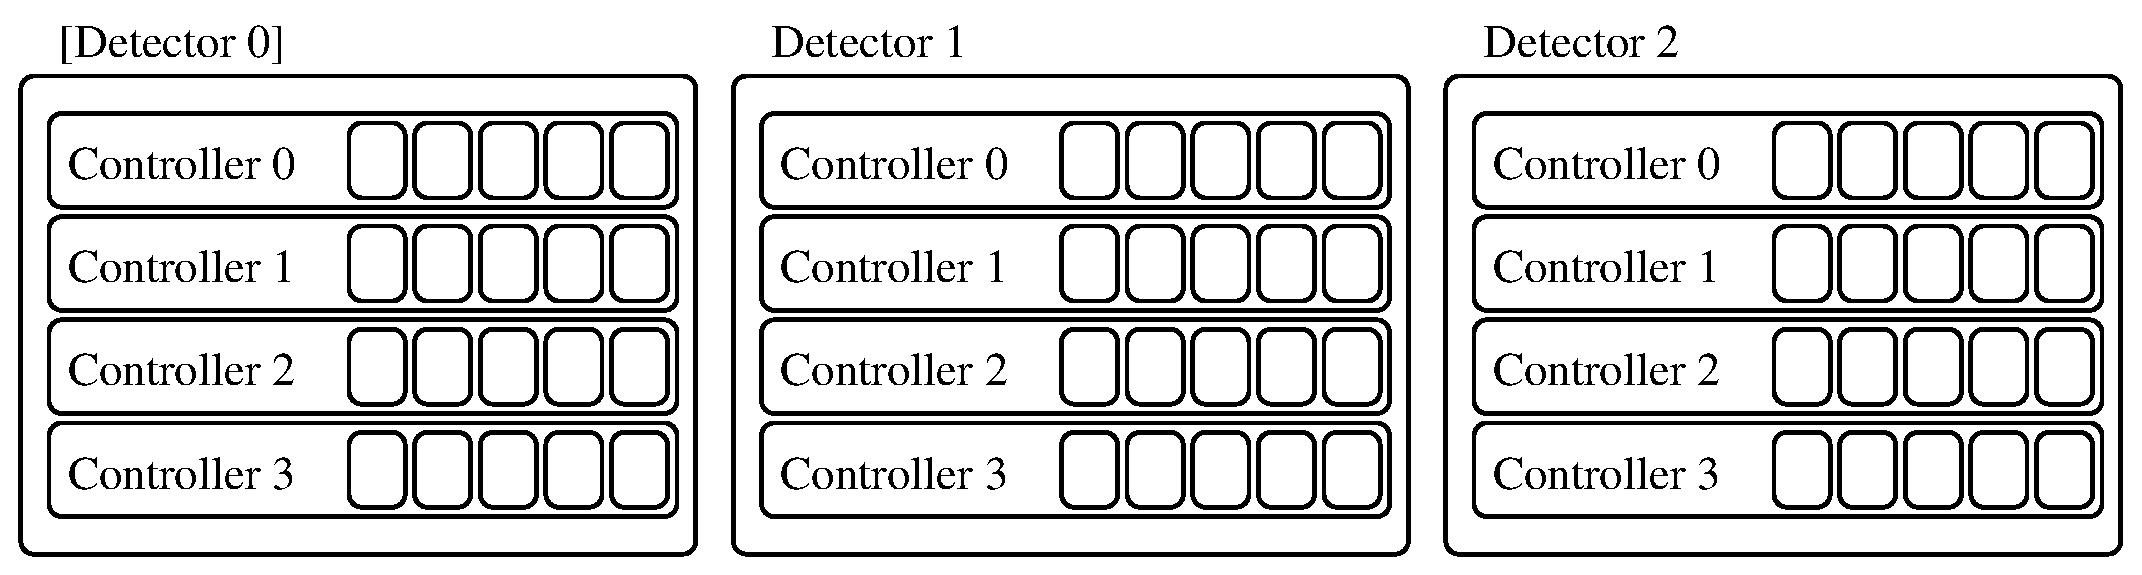
\includegraphics[width=\textwidth]{multi_detector}
\end{figure} 

\subsubsection{Examples}

For MYTHEN, if one needs to control 6 modules, the system can either be composed by and MCS6 with 6 modules (1 detector, 1 controller, 6 modules), or by 6 MCS1 (1 detector, 6 controller, 1 module each). After apppropriate configuration of the system, the interface to the user will be the same for both systems.

For GOTTHARD, one module corresponds to one controller. A detector will have the smae number of controllers and modules.

For EIGER, one module consists in two controllers. Fo a multi-module system, the number of controllers will increase accordingly, but should be left to a configuration file.

You will need to configure more than one detector, only in case you want to operate several detectors independently.


\subsection{How can I configure the data receiver?}

For slower acquisitions, the detector will return the data to the control PC over TCP/IP (e.g. MYTHEN).

However, for faster frame rates (e.g. GOTTHARD, EIGER) the controllers will return the data to a data receiver i.e. a process specifically designed to receive the data from the controller over a GBit network and save them to disk. \\
The data receiver can run on any machine (e.g. a file server) accessible by both the control PC and the detector controller, as sketched in figure~\ref{fig:datareceiver}.

After starting the data receiver process and correctly configuring the client and the detector, this architecture should be completely transparent for the user, except that the output file path must be properly configured from the client for the data receiver machine (easiest is that the disk is mounted for both machines in the same location).\\
The cleint will take care of communicating with the data receiver and the detector. A feedback about the progress of the acquisition and a preview of the data being acquired can also be obtained by the client from the data receiver.


\begin{figure}
\caption{Scketch of the comminication between the control PC, the detector and the data receiver.}\label{fig:datareceiver}
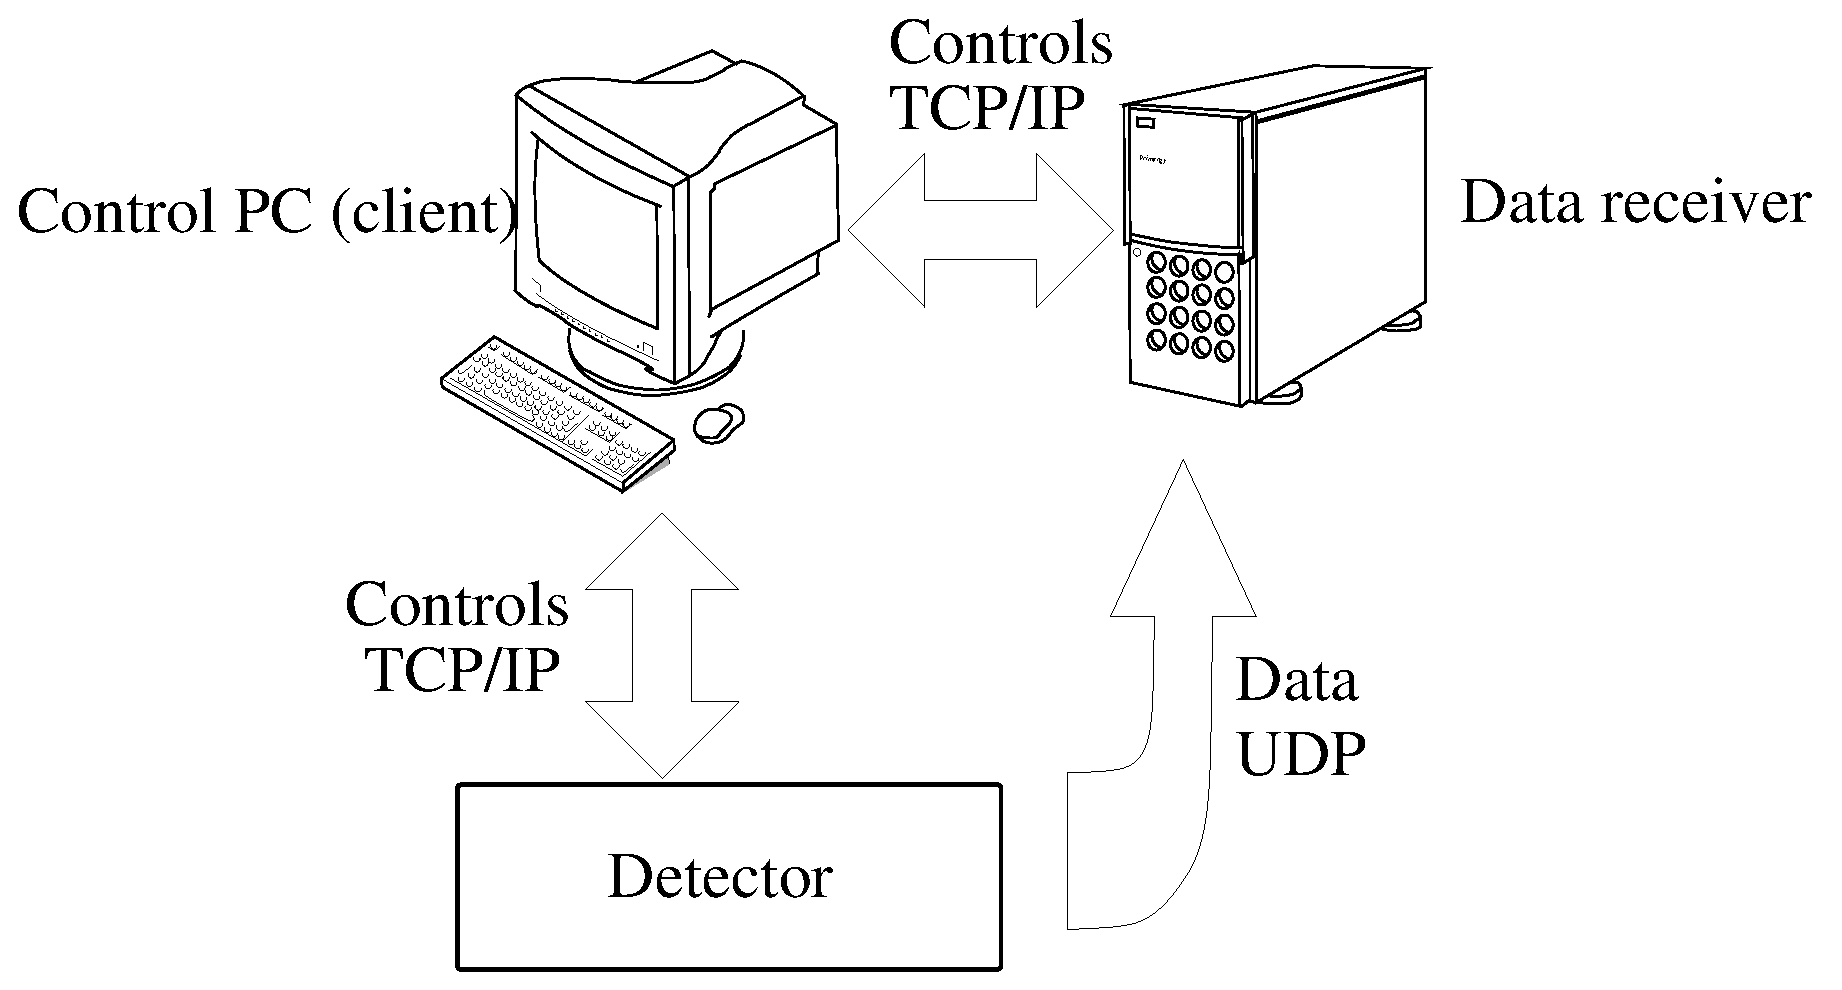
\includegraphics[width=\textwidth]{data_receiver}
\end{figure} 

\subsection{What are settings and calibration files for?} \label{sec:trimdir}


\subsubsection{MYTHEN}
In order to be able to properly operate your detector you need a directory where the trimbit files (needed to set the detector settings and eventually equalize the individual channel thresholds) which in the following will be named \textit{settingsdir} and a directory where the calibration files (needed to convert the threshold energy in DAC units) are stored which in the following will be named \textit{caldir}. \\
\textit{settingsdirdir} and \textit{caldir} can even be the same directory, and an example of it is given in the software package by the example directory \verb=trimdir=. 
Since these directories are customized by producing trimbit files and calibration for each detector, make sure not to overwrite yours every time you upgrade the software.

\textit{settingsdir} should contain three subdirectories \verb=standard=,  \verb=fast= and  \verb=highgain= containing respectively the trimfiles \verb=standard.trim=,  \verb=fast.trim= and  \verb=highgain.trim= which contain the correct voltage settings for the detector although all the individual channel thresholds set to 0. The original files contained in the package should be used, infact in case of error the detector would not recognize the correct settings.\\
The default trimbit files for each file will be stored in the directory according to the settings with the name \verb=noise.snxxx= where \verb=xxx= is the module serial number.\\

\textit{caldir} should contain three subdirectories \verb=standard=,  \verb=fast= and  \verb=highgain= containing respectively the trimfiles \verb=standard.cal=,  \verb=fast.cal= and  \verb=highgain.cal= which contain an average calibration of the modules for the diffrent settings. However this can different from the correct one for each individual module even of several kev and therefore it is very important to perform an energy calibration on a module basis.\\
The default calibration files for each file will be stored in the directory according to the settings with the name \verb=calibration.snxxx= where \verb=xxx= is the module serial number.

The \textit{settingsdir} and \textit{caldir} should be properly configured for your detector either in a configuration file (for use with text clients, GUI or API) or dynamically (works only for the text clients).

\subsubsection{GOTTHARD}
A \textit{settingsdir} should be configured, as the directory  \verb=settings= in this software package.\\
It must contain the subdirectories \verb=dynamicgain=, \verb=gain1=,  \verb=gain2=,  \verb=gain3=,  \verb=highgain=,  \verb=lowgain=,  \verb=mediumgain=, and   \verb=veryhighgain= in order to properly configure the GOTTHARD detector using the various gain settings.


\subsection{How should a configuration file look like?}


\subsection{What is the meaning of the file name?}
The final file name will be: \\
\textit{outdir/prefix}\verb=[_d=$d$\verb=][_S=\textit{v0}\verb=][_s=\textit{v1}\verb=][_p=\textit{p}\verb=][_f=\textit{f}\verb=]_=\textit{i}\verb=.=\textit{ext}\\
where: \\
\textit{outdir} is the output directory path;\\
\textit{prefix} is the chosen prefix for the file name;\\
\textit{d} is the detector index, in case of data receiver and more than one detector;\\
\textit{v0} is the scan0 variable with the desired precision, if scan0 is enabled;\\
\textit{v1} is the scan1 variable with the desired precision, if scan1 is enabled;\\
\textit{p} is the position index, if different positions are configured;\\
\textit{f} is the frame index of the first frame stored in the file, if many frames and cycles are configured;\\
\textit{i} is the file index;\\
\textit{ext} is the file extension e.g. \textit{.raw} for MYTHEN raw data, \textit{.dat} for MYTHEN processed data.

\subsection{Which is the sequence of the acquisition flow?}

       case startScript:
       case stopScript:
 nrun=i par=p

     case scriptBefore: 
     case scriptAfter: 
nrun=i fn=fn par=p sv0=v0 sv1=v1 p0=p0 p1=p1
   
     case headerBefore:
     case headerAfter: nrun=i fn=fn par=p

case scan:
 nrun=i fn=fn var=v par=p



\begin{displaymath}
%%%%%%%%%%%%%%%%%%%%%8
  \textrm{Measurement loop} \\
 \left\{ \qquad
    \begin{array}{l} \\
  %   \textrm{Measurement loop} \\
     \\
%%%%%%%%%%%%%%%%%%%%%7
    % \left[ 
     \qquad
           \begin{array}{l} \\
        	  \blacksquare  \,  \textrm{Start script} \\
	   \\
%%%%%%%%%%%%%%%%%%%%%6
                   \textrm{Scan 0 loop}
           \left\{  
     \qquad
	          \begin{array}{l} \\
           %        \textrm{Scan 0 level} \\
		   \\
%%%%%%%%%%%%%%%%%%%%%5
     
                   \textrm{Scan 1 loop}      \left\{  
     \qquad
	          \begin{array}{l} \\
                %   \textrm{Scan 1 level} \\
		   \\
%%%%%%%%%%%%%%%%%%%%%4
          % \left[  
     \qquad
	          \begin{array}{l} \\
                 	  \blacksquare \,  \textrm{Script before} \\
		   \\
%%%%%%%%%%%%%%%%%%%%%3
           \left\{  
     \qquad
	          \begin{array}{l} \\
                   \textrm{Position loop} \\
		   \\
%%%%%%%%%%%%%%%%%%%%%2
         %  \left[  
     \qquad
	          \begin{array}{l} \\
             	  \blacksquare \,     \textrm{Header before} \\
		   \\
%%%%%%%%%%%%%%%%%%%%%1
           \left\{  
     \qquad
	          \begin{array}{l} \\
                  \textrm{Cycles loop} \\
		  \\
%%%%%%%%%%%%%%%%%%%%%0
           \left\{  
     \qquad
	          \begin{array}{l}
		   \\
                   \textrm{Frames loop} \\
		   \\
                   \end{array}
	   \right. \\ 
	   \\
%%%%%%%%%%%%%%%%%%%%%%%%%%0
\\
           \end{array}
	   \right. \\ 
	   \\
%%%%%%%%%%%%%%%%%%%%%%%%%%1
        	  \blacksquare \,  \textrm{Header after}\\
\\
           \end{array}
	 %  \right. \\ 
%%%%%%%%%%%%%%%%%%%%%%%%%%2
\\
           \end{array}
	   \right. \\ 
	   \\
%%%%%%%%%%%%%%%%%%%%%%%%%%3
	  \blacksquare \, \textrm{Script after} \\
\\
                   \end{array}
	  % \right. \\ 
	   \\
%%%%%%%%%%%%%%%%%%%%%%%%%%4
\\
                   \end{array}
	   \right. \\ 
%%%%%%%%%%%%%%%%%%%%%%%%5
\\
                   \end{array} 
	   \right. \\
	   \\
%%%%%%%%%%%%%%%%%%%%%%%%6
	  \blacksquare	\,   \textrm{Stop script} \\
\\
            \end{array} 
 %     \right. \\
      \\
%%%%%%%%%%%%%%%%%%%%%%%%7
\\
      \end{array}  
\right. 
%%%%%%%%%%%%%%%%%%%%%%%%8
\end{displaymath}




\subsection{How can I synchronize my detector wit the experiment?}

\begin{figure}
\begin{center}
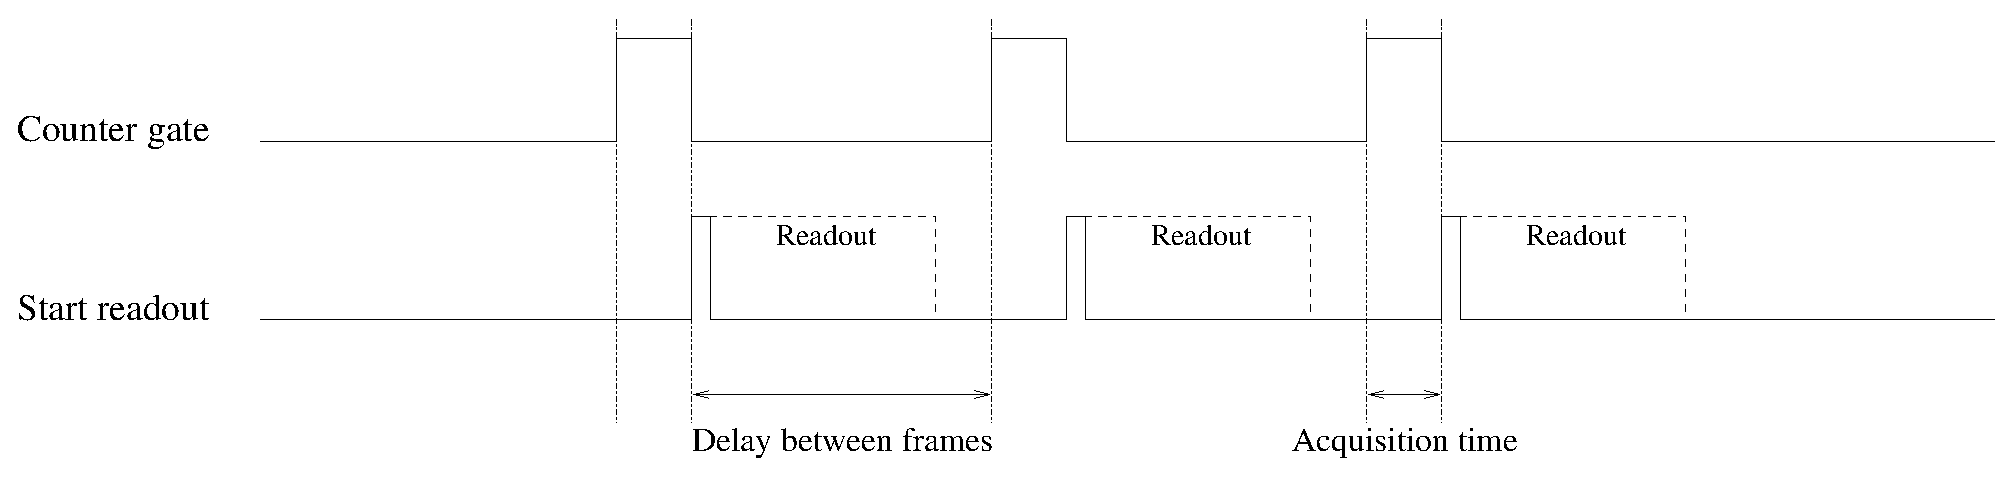
\includegraphics[width=\textwidth]{images/normal_acquisition.eps}
\end{center}
\caption{Auto timing}\label{fig:autotiming}
\end{figure}

\begin{figure}
\begin{center}
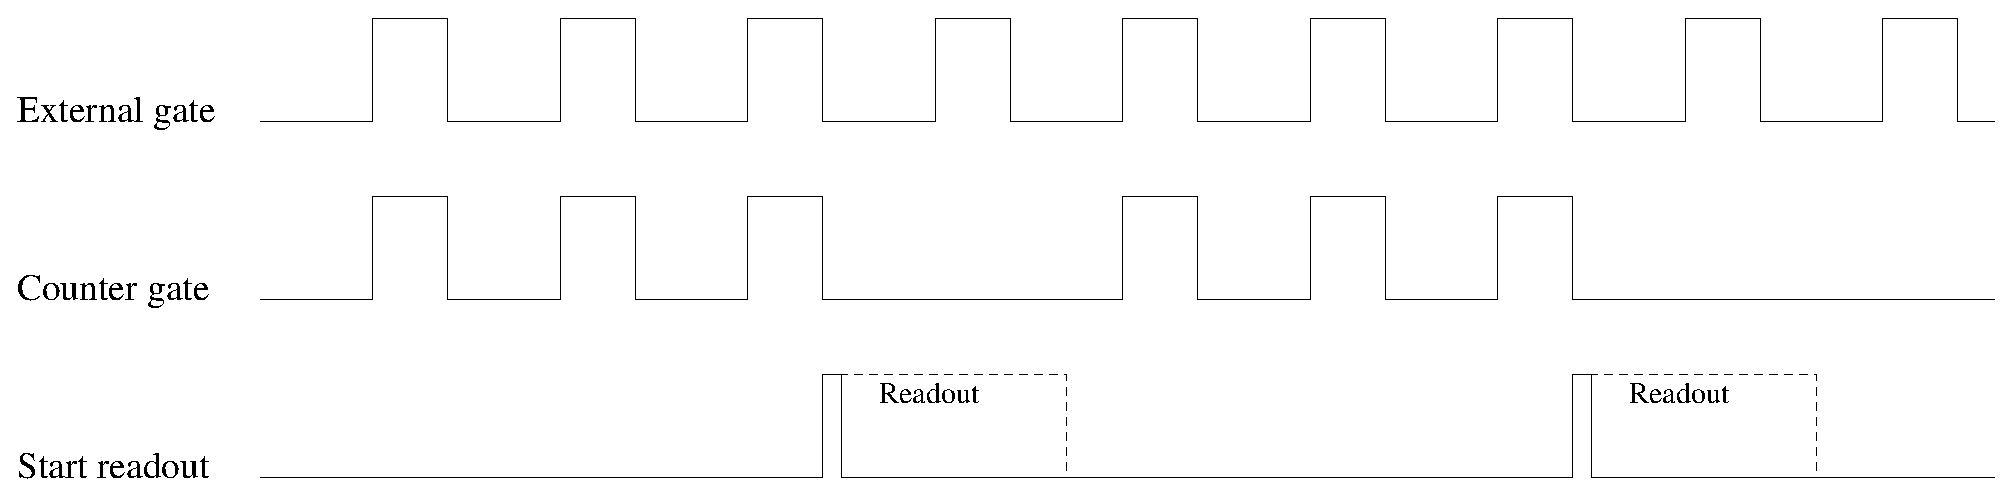
\includegraphics[width=\textwidth]{images/gated_acquisition.eps}
\end{center}
\caption{Gating}\label{fig:gating}
\end{figure}

\begin{figure}
\begin{center}
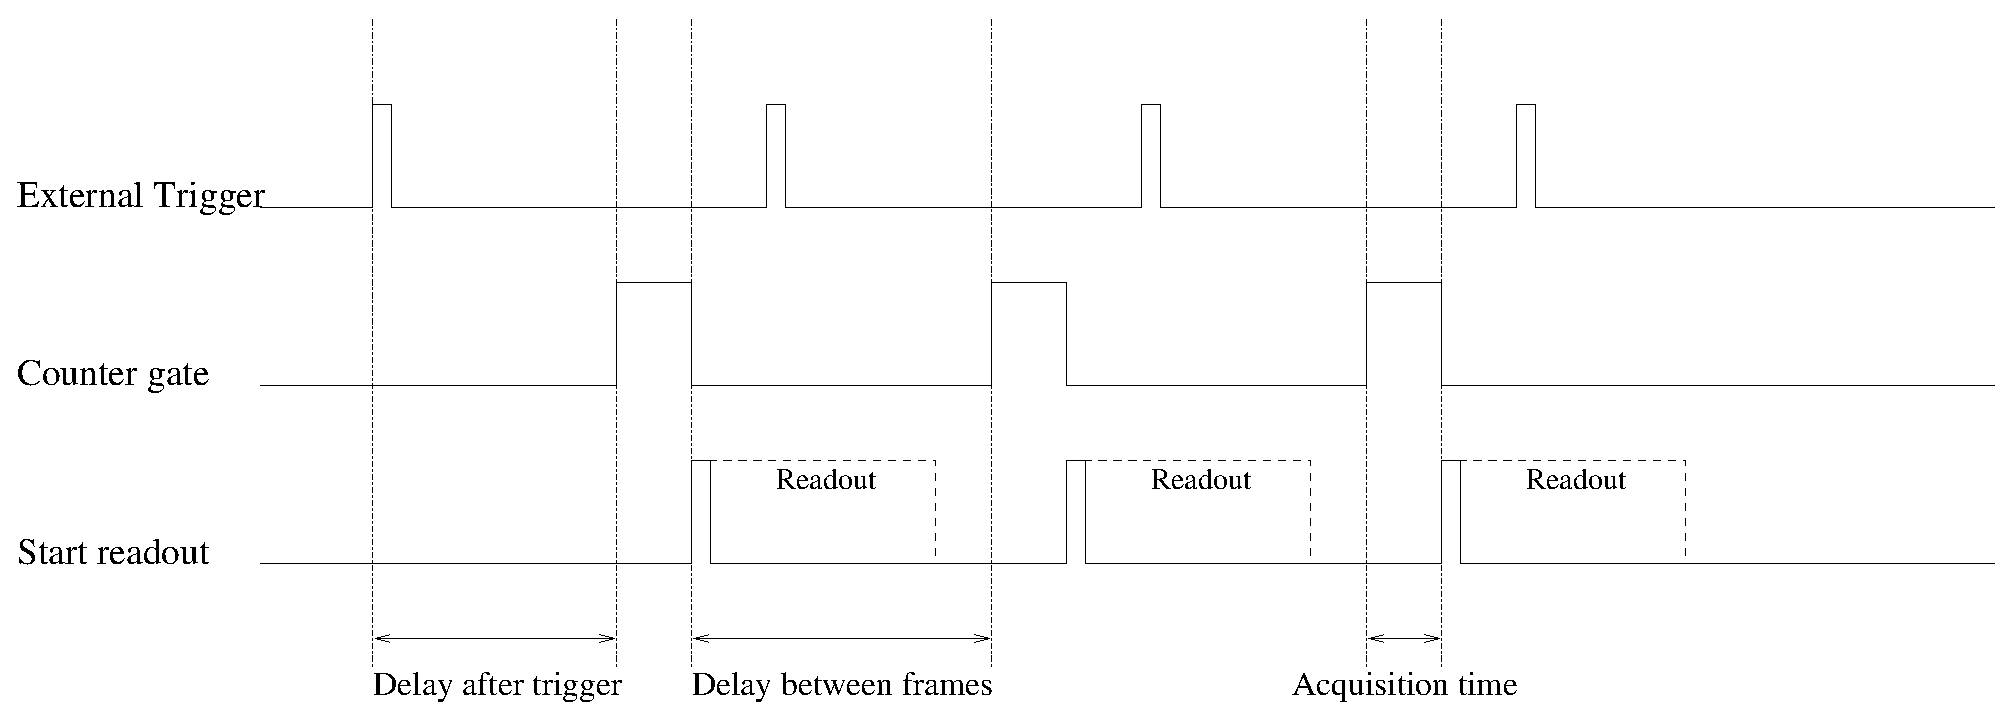
\includegraphics[width=\textwidth]{images/single_trigger_acquisition.eps}
\end{center}
\caption{Single trigger}\label{fig:singtrig}
\end{figure}

\begin{figure}
\begin{center}
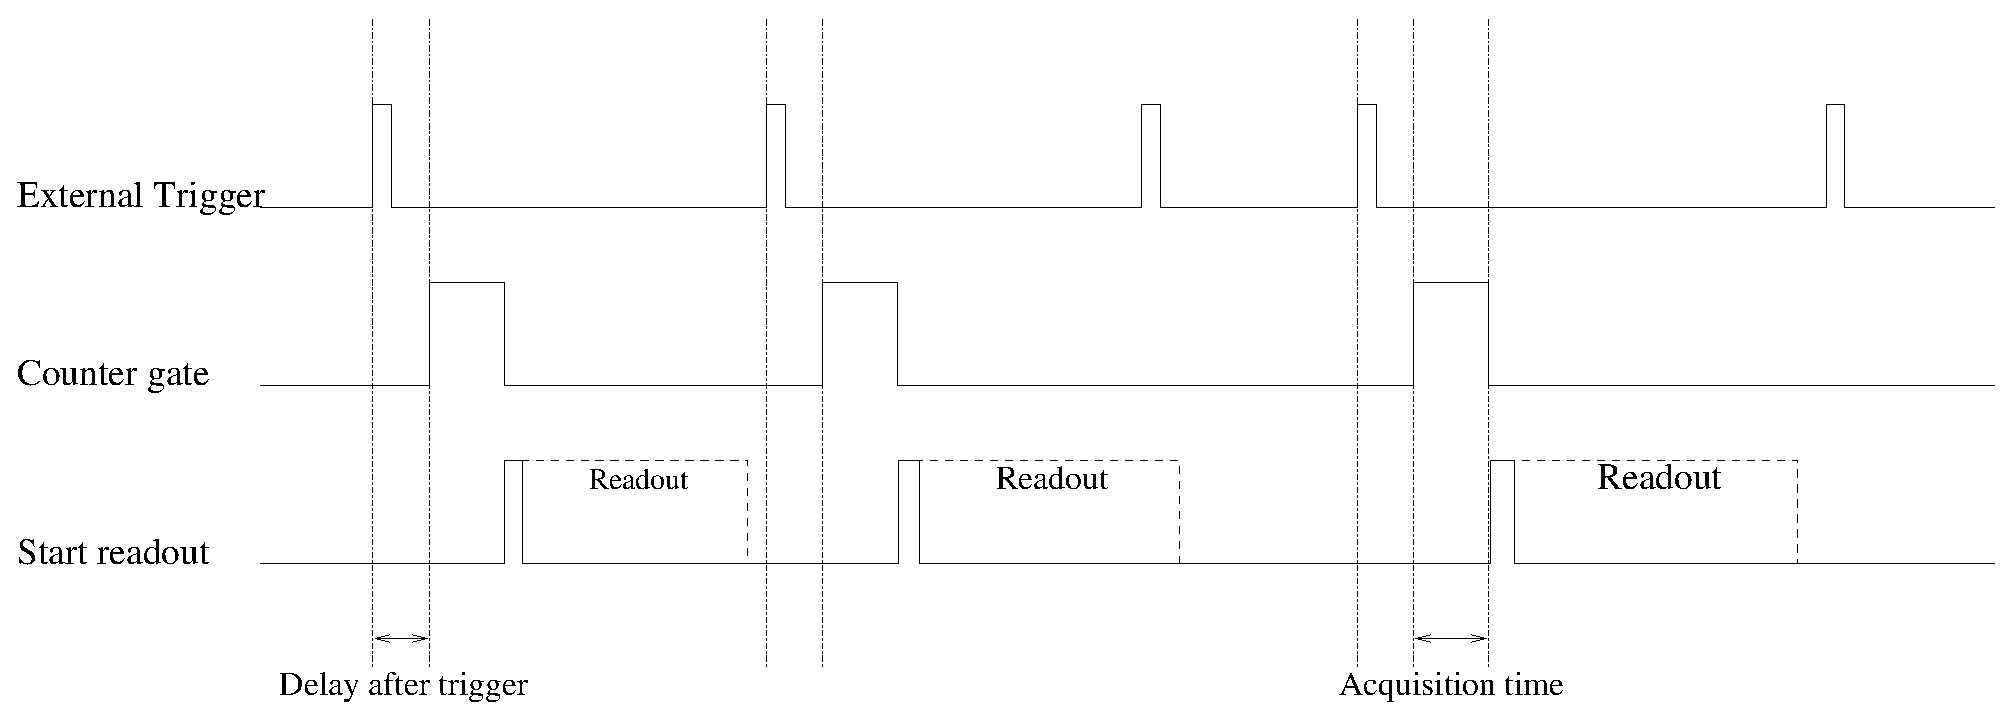
\includegraphics[width=\textwidth]{images/continuos_trigger_acquisition.eps}
\end{center}
\caption{Continous trigger}\label{fig:conttrig}
\end{figure}



\subsubsection{How do I synchronize several controllers?}

\subsubsection{How do I move the detector and read the encoder for angular conversion or read my intensity monitor for intensity normalization?}



\section{General questions about detectors}


\subsection{In which X-ray energy range can I use the detector?}

General remarks about sensor efficiency and electronic noise

\subsection{What is the electronic noise?}\label{sec:noise}


\subsection{What limits the maximum frame rate?}


\section{Single photon counting detectors}





\subsection{Which detector settings should I choose?}

The choice of the operation settings is very important in order to obtain good quality data. 


Normally the user can follow these rules:
\begin{enumerate}
\item If the X-ray energy is lower than 8~keV the \textit{High gain} setting should be used. Since it is a slow mode of operation it is necessary to take care that the maximum count rate is lower than 100~kcounts/s for all channels (use filters to reduce the beam intensisty).
\item For energies higher than 8~keV, the \textit{Standard} setting is normally fine if the count rate can be kept lower than 300~kcounts/s for all channels (use filters to reduce the beam intensisty). 

\item In case a larger count rate is required in order to keep the acquisition time shorter, the \textit{Fast} setting must be selected. However the maximum count rate should never exceed 1~Mcounts/s   for all channels.
\end{enumerate}

\subsubsection{MYTHEN}


\begin{figure}
\begin{center}
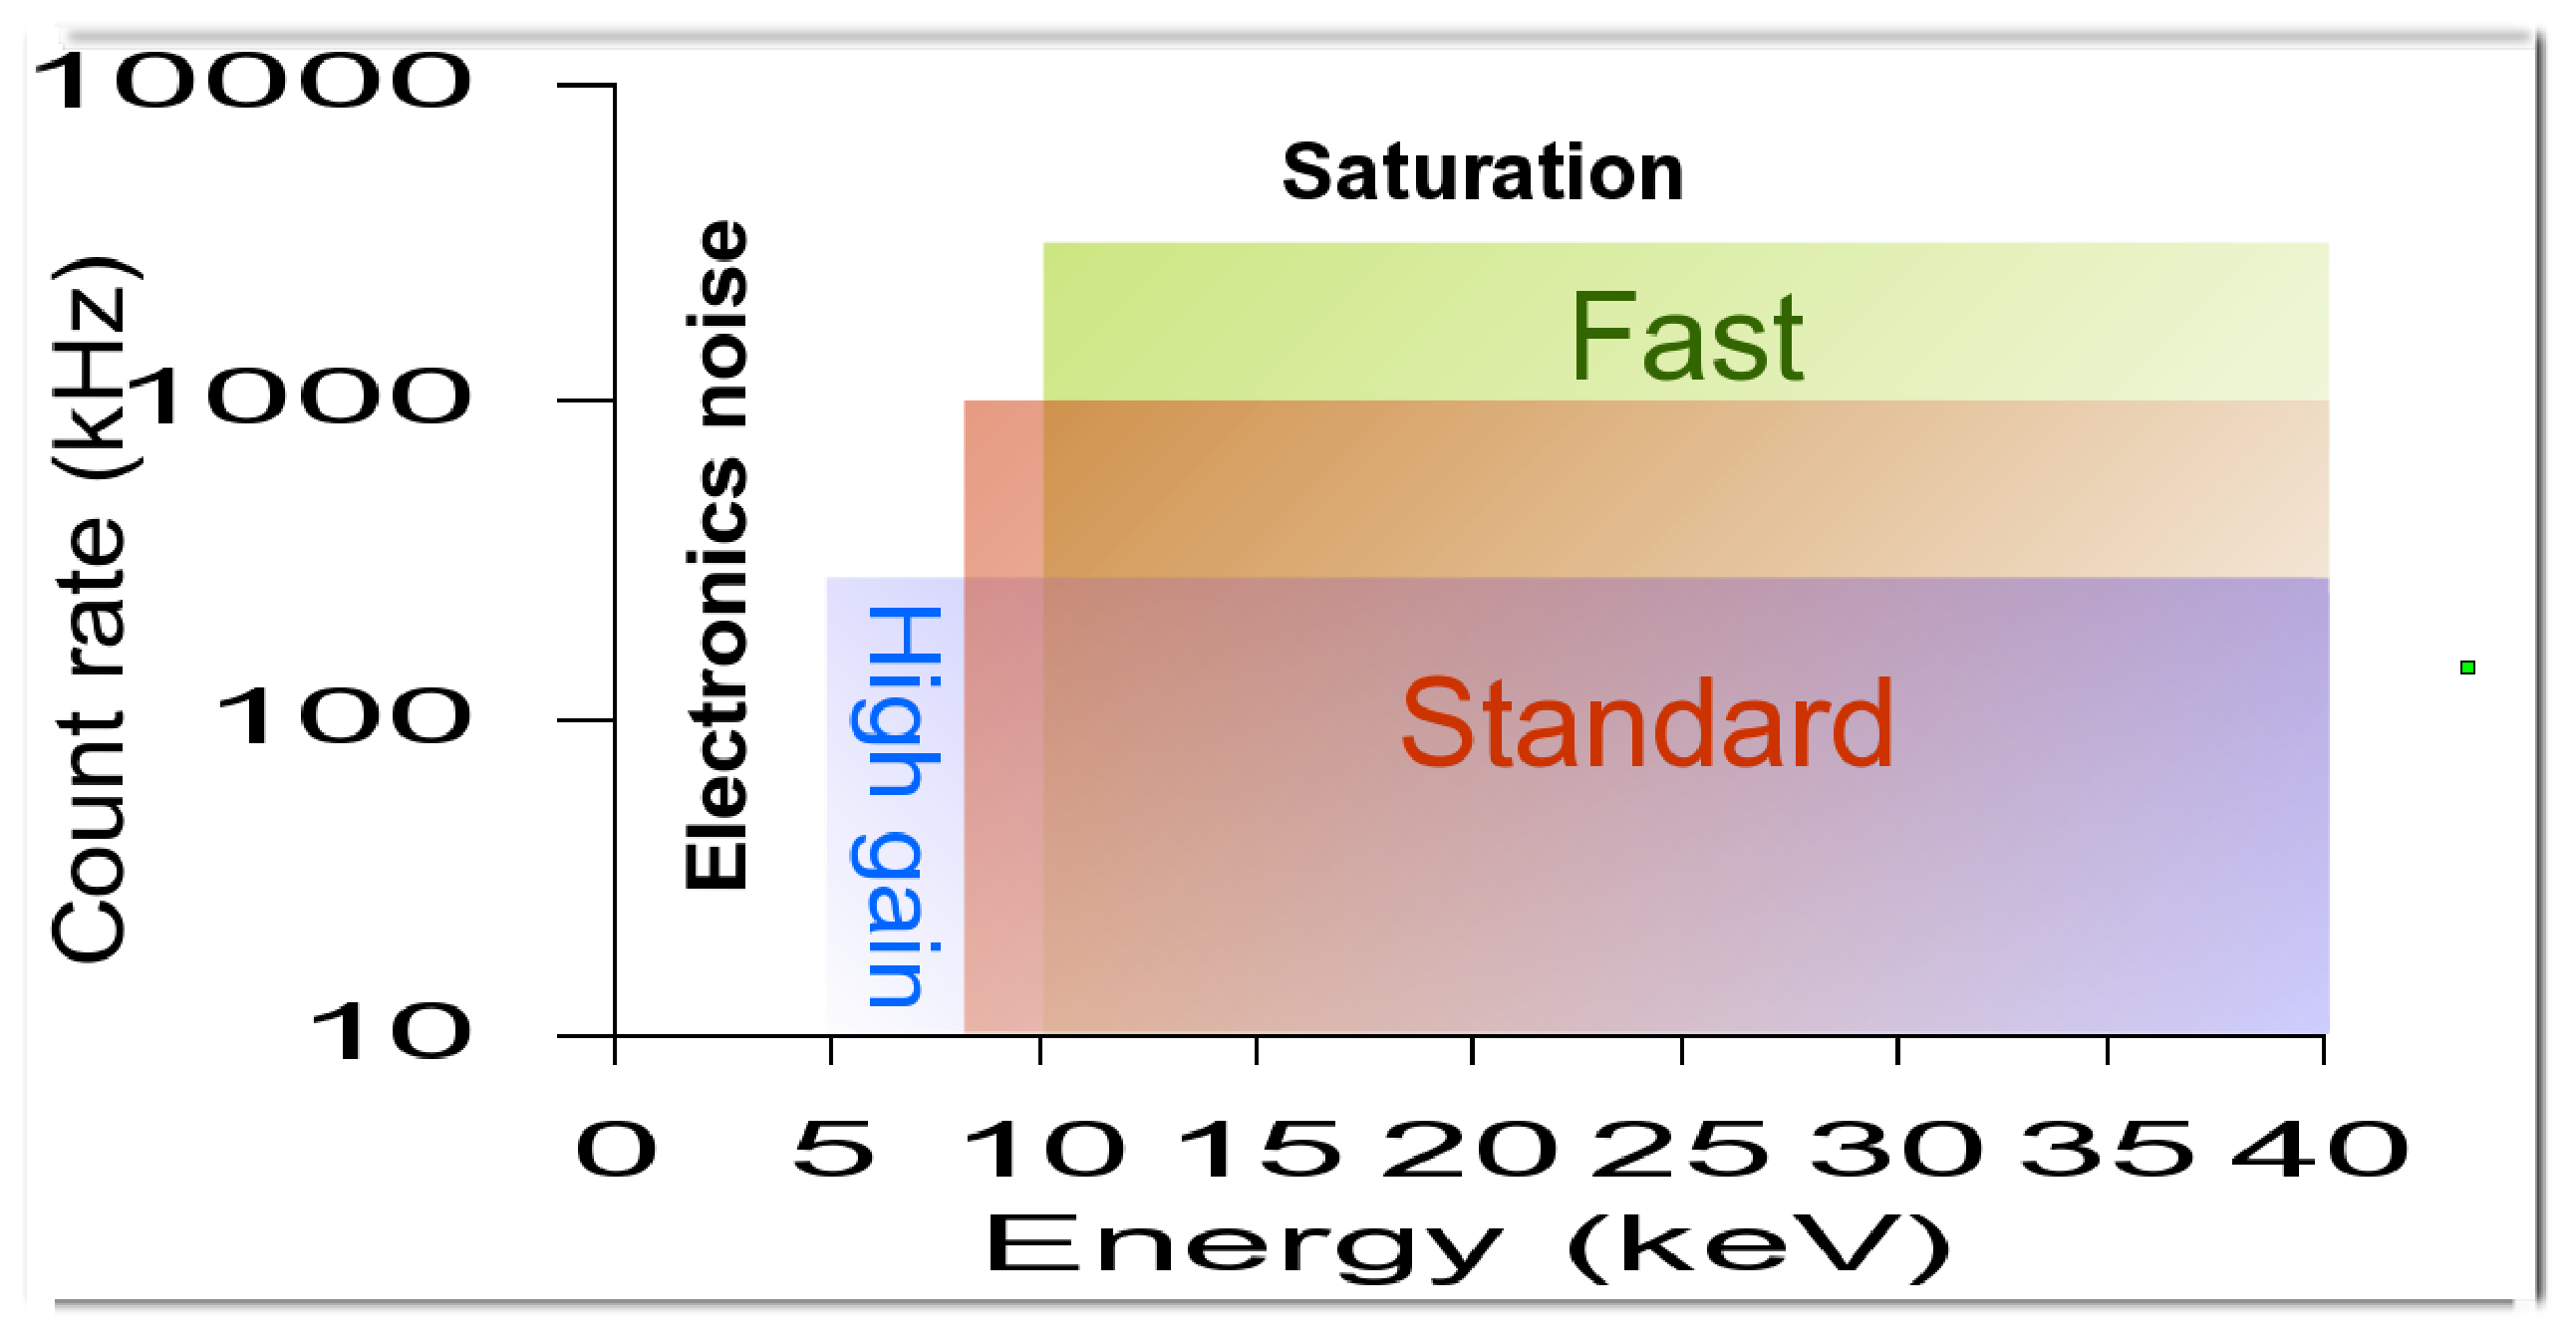
\includegraphics[width=\textwidth]{images/settings}
\end{center}
\caption{Plot indicating the reccomended choice of detector settings as a function of the X-ray energy and maximum count rate per channel..}\label{fig:settings}
\end{figure}


\subsection{How do I chose the comparator threshold?}

\begin{figure}[b!]
\begin{center}
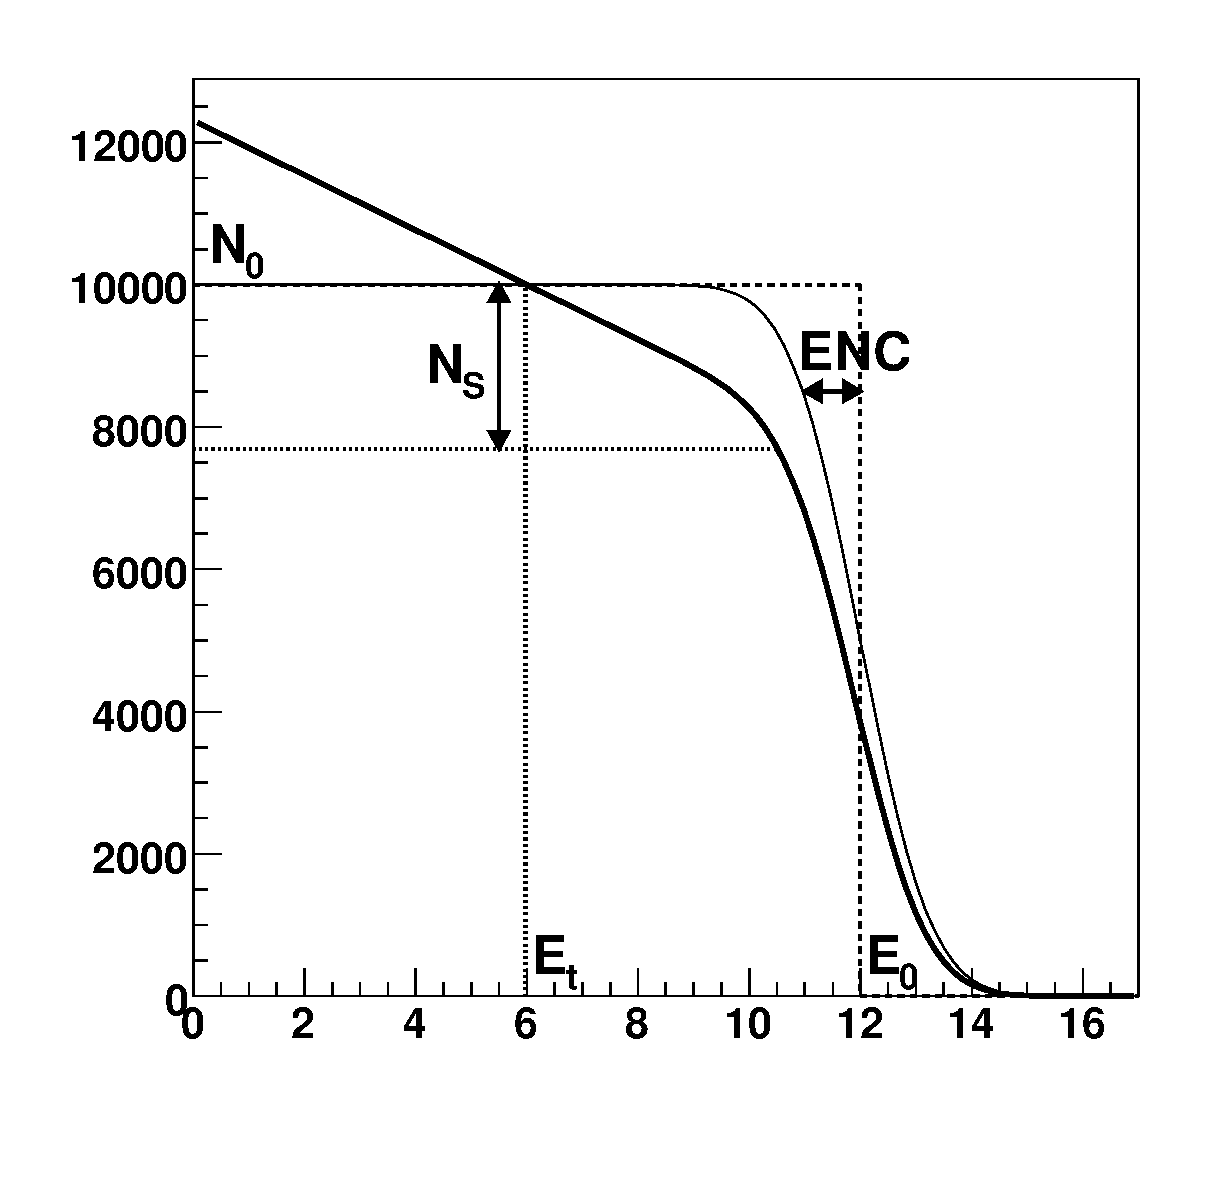
\includegraphics[width=\textwidth]{images/thr_scan_expl}
\end{center}
\caption{Number of counts as a function of the threshold detected in an ideal case.}\label{fig:thrscan}
\end{figure}

\begin{figure}[t!]
\begin{center}
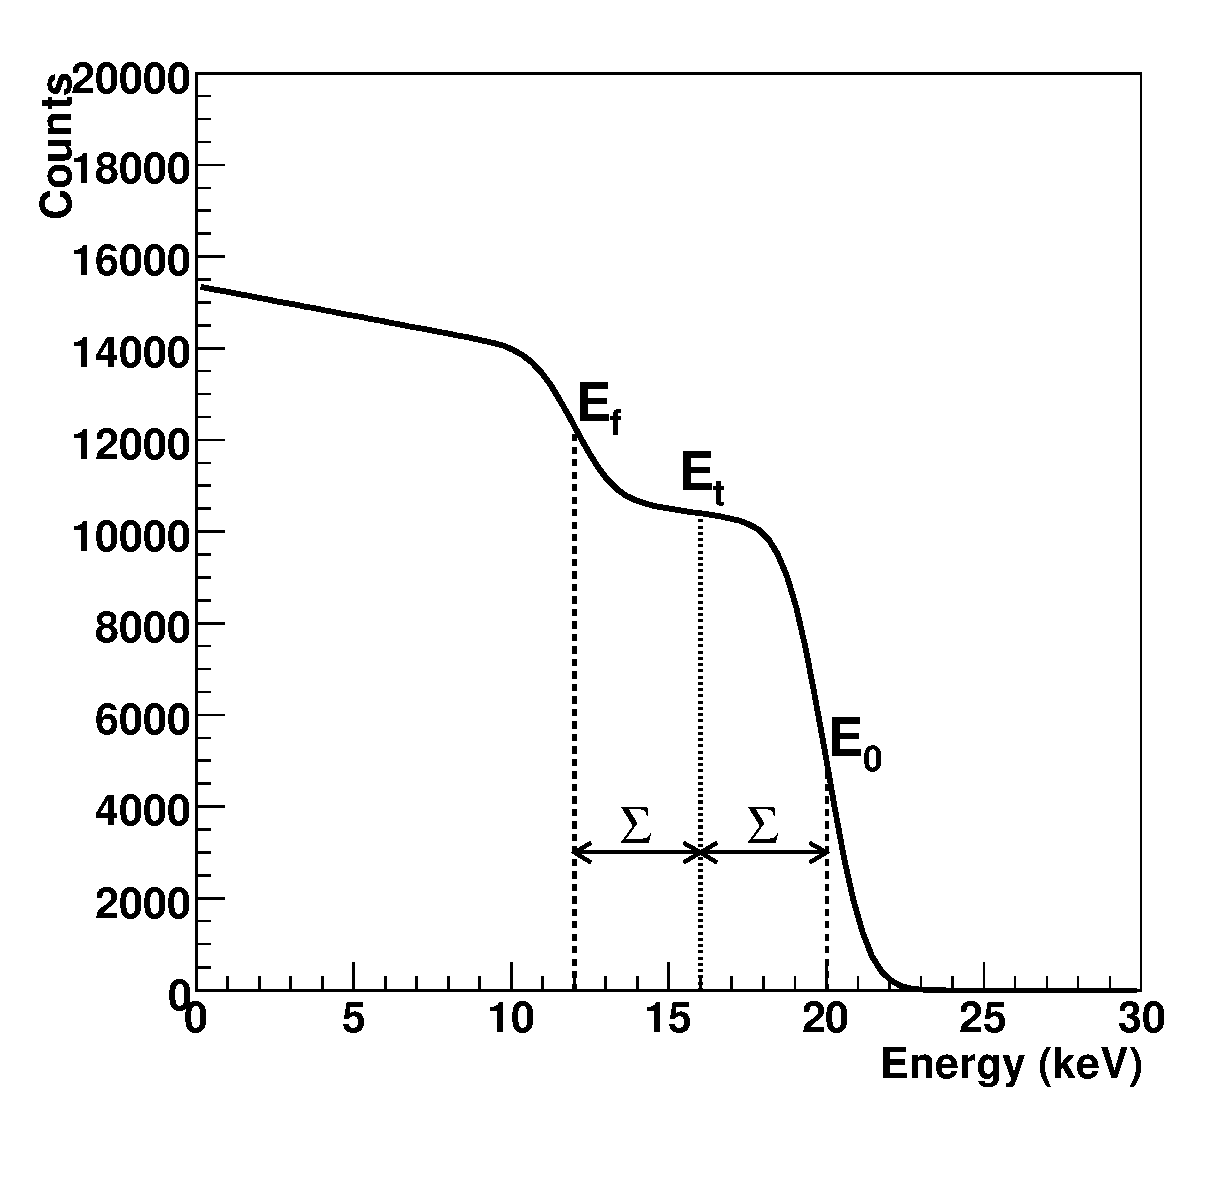
\includegraphics[width=\textwidth]{images/thr_scan_fluo}
\end{center}
\caption{Number of counts as a function of the threshold detected in presence of fluorescent radiation}\label{fig:thrscanfluo}
\end{figure}

Once selected the settings, the threshold should be selected.
Figure~\ref{fig:thrscan} shows the number of counts as a function of the threshold value in the ideal case of monoenergetix X-rays of energy $E_0$=10~keV.
For thresholds larger than the X-ray energy the detector should always count 0 and for lower thresholds it should always count all the photons. However the curve is smoothed around $E_0$ because of the electronic noise (ENC) and is not perfectly flat for lower energies because the photons absorbed in the region between two strips distribute their energy between them and it is not flully collected by a single channel (charge sharing).\\
In order to count once al X-rays the threshold should be set at half of the X-ray energy $E_t=E_0/2$: if the threshold would be higher some photons would not be counted, leading to a loss of efficiency, while if it would be lower some photons would be counted twice leading to a loss of spatial resolution. 

Since the detector threshold can't be precisely set at the same value for all channels but there will always be some spread of the order of 200~eV (threshold dispersion) there will always be some fluctuations on the number of counts between channels, which however should be corrected by the flat field correction.

The choice of the threshold should also depend from  considerations regarding the emission of fluorescent radiation from the sample.\\
Figure~\ref{fig:thrscanfluo} shows  how the curve of the counts would look like for monochromatic X-rays of energy $E_0$ in presence of radiation of energy $E_f$ emitted by the sample. The curve would show a second step at $E_f$. 

Since the fluorecence emission is not present in the flat field data, the difference of counts between the channels due to the fluorescent radiation cannot be corrected and the threshold $E_t$ should be set at an energy larger than $E_f$. This also helps to cut down the background.\\
The difference of counts between the channels will be particularly large if the threshold is set in some ``steep'' part of the curve i.e. close to $E_f$ or to $E_0$ (but in this case it would be corrected by the flat field, at cost of loss of efficiency).
Because of the presence of the electronic noise, $E_t$ should be at least 3~keV larger than $E_f$.

Here is a short list of rules to select the appropriate working threshold in order of importance (and eventually modify the X-ray energy):
\begin{enumerate}
\item List the fluorescent emission lines $E_f$ that you expect from your sample. 
\item If there is no fluorescent emission ($E_f<E_0$) $E_t=E_0/2$
\item If there is fluorescent emission 
\begin{enumerate}
\item $E_t>E_f+3$~keV
\item $E_t<E_0-3$~keV 
\end{enumerate}
If the range where both requirements are satisfied is large, try to increase the distance of $E_t$ from $E_f$ up to 5~keV and then set $E_t$ as close as possible to the ideal value $E_t=E_0/2$
\item If it is not possible to satisfy the previous minimal requirements:
\begin{enumerate}
\item If you need high quality data and you can sacrifice detector efficiency (a lot!)  $E_t>E_f+3$~keV
\item If you need fast measurments and you can sacrifice detector uniformity (difficult to say how much) and increase the background $E_t<E_f-3$~keV. Remember that $E_t$ is klimited by the electronic noise $E_t>4$~keV (3~keV for \textit{High gain} settings).
\item Consider to change $E_0$ to values lower than $E_f$ or at least 6-8~keV larger than $E_f$ 
\end{enumerate}
\end{enumerate}



\begin{figure}
\begin{center}
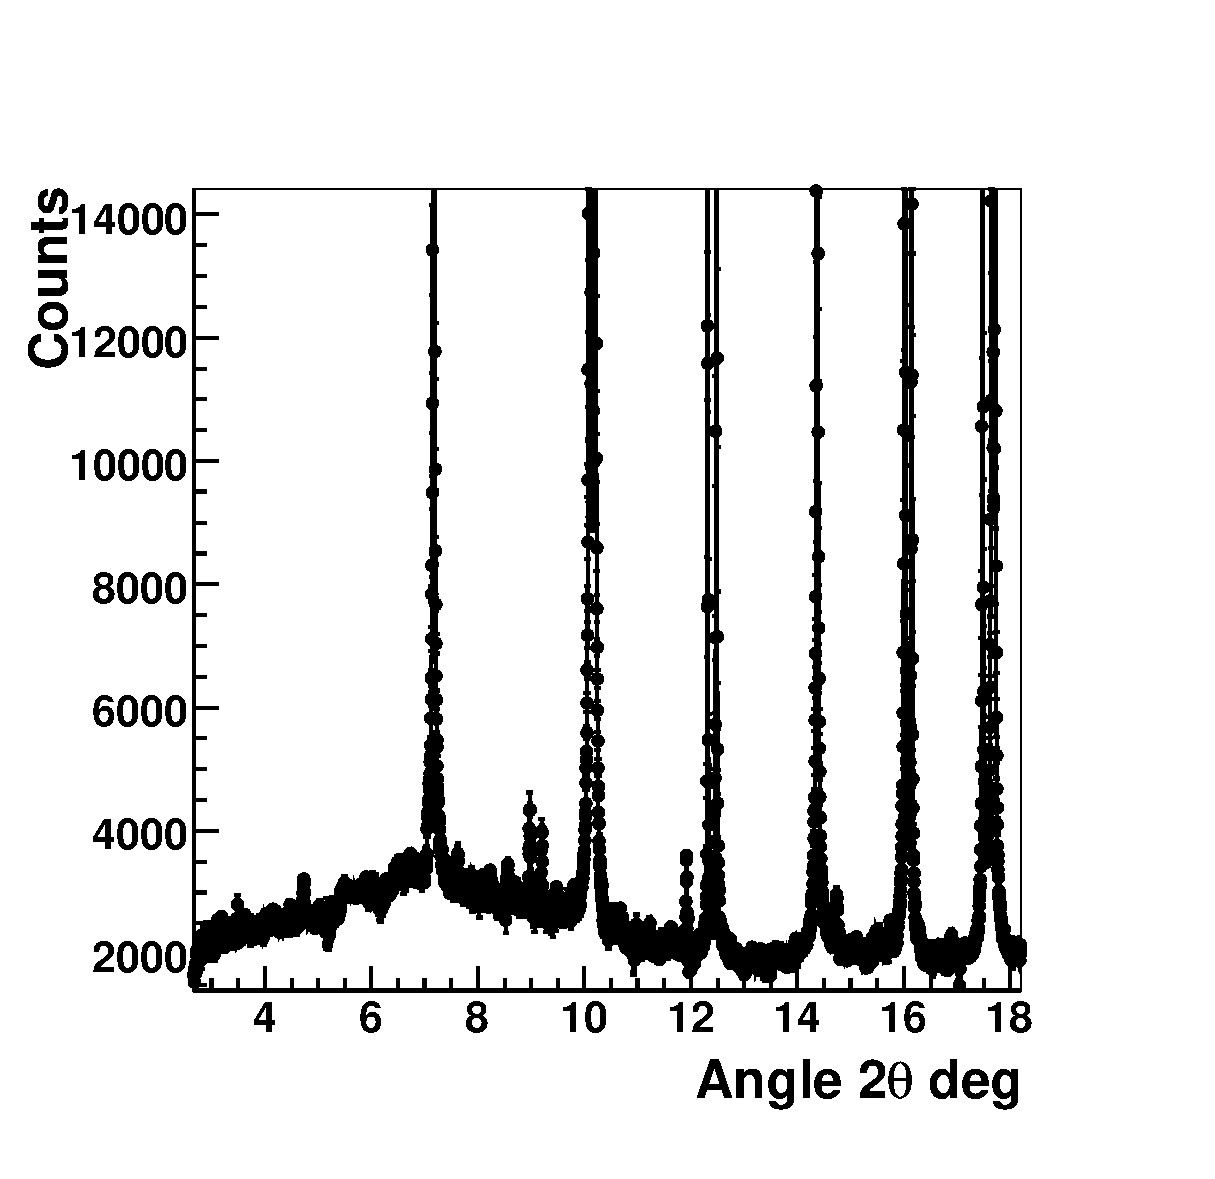
\includegraphics[width=\textwidth]{images/sample_with_fluorescence}
\end{center}
\caption{Example of data from a sample emitting fluorescent light and detector threshold set at a value close to the emission line. The background data cannot be properly flat field corrected.}\label{fig:samplefluo}
\end{figure}


\subsection{Why isn't my flat-field flat?}

The main reasons of a non flat flat-field can be:
\begin{itemize}
\item The scattering from the glass rod is not uniform over the angular range. In this case you should take the flat field dynamically i.e. scanning the detector in front of the cylinder with the small window, as we do at the SLS. In this case when you shift the detector, the shape of the illumination remains in the same angular position (and shifts in channel number). Of course it depends a lot on the energy and on the geometry of the flat field acquisition.
\begin{figure}
\begin{center}
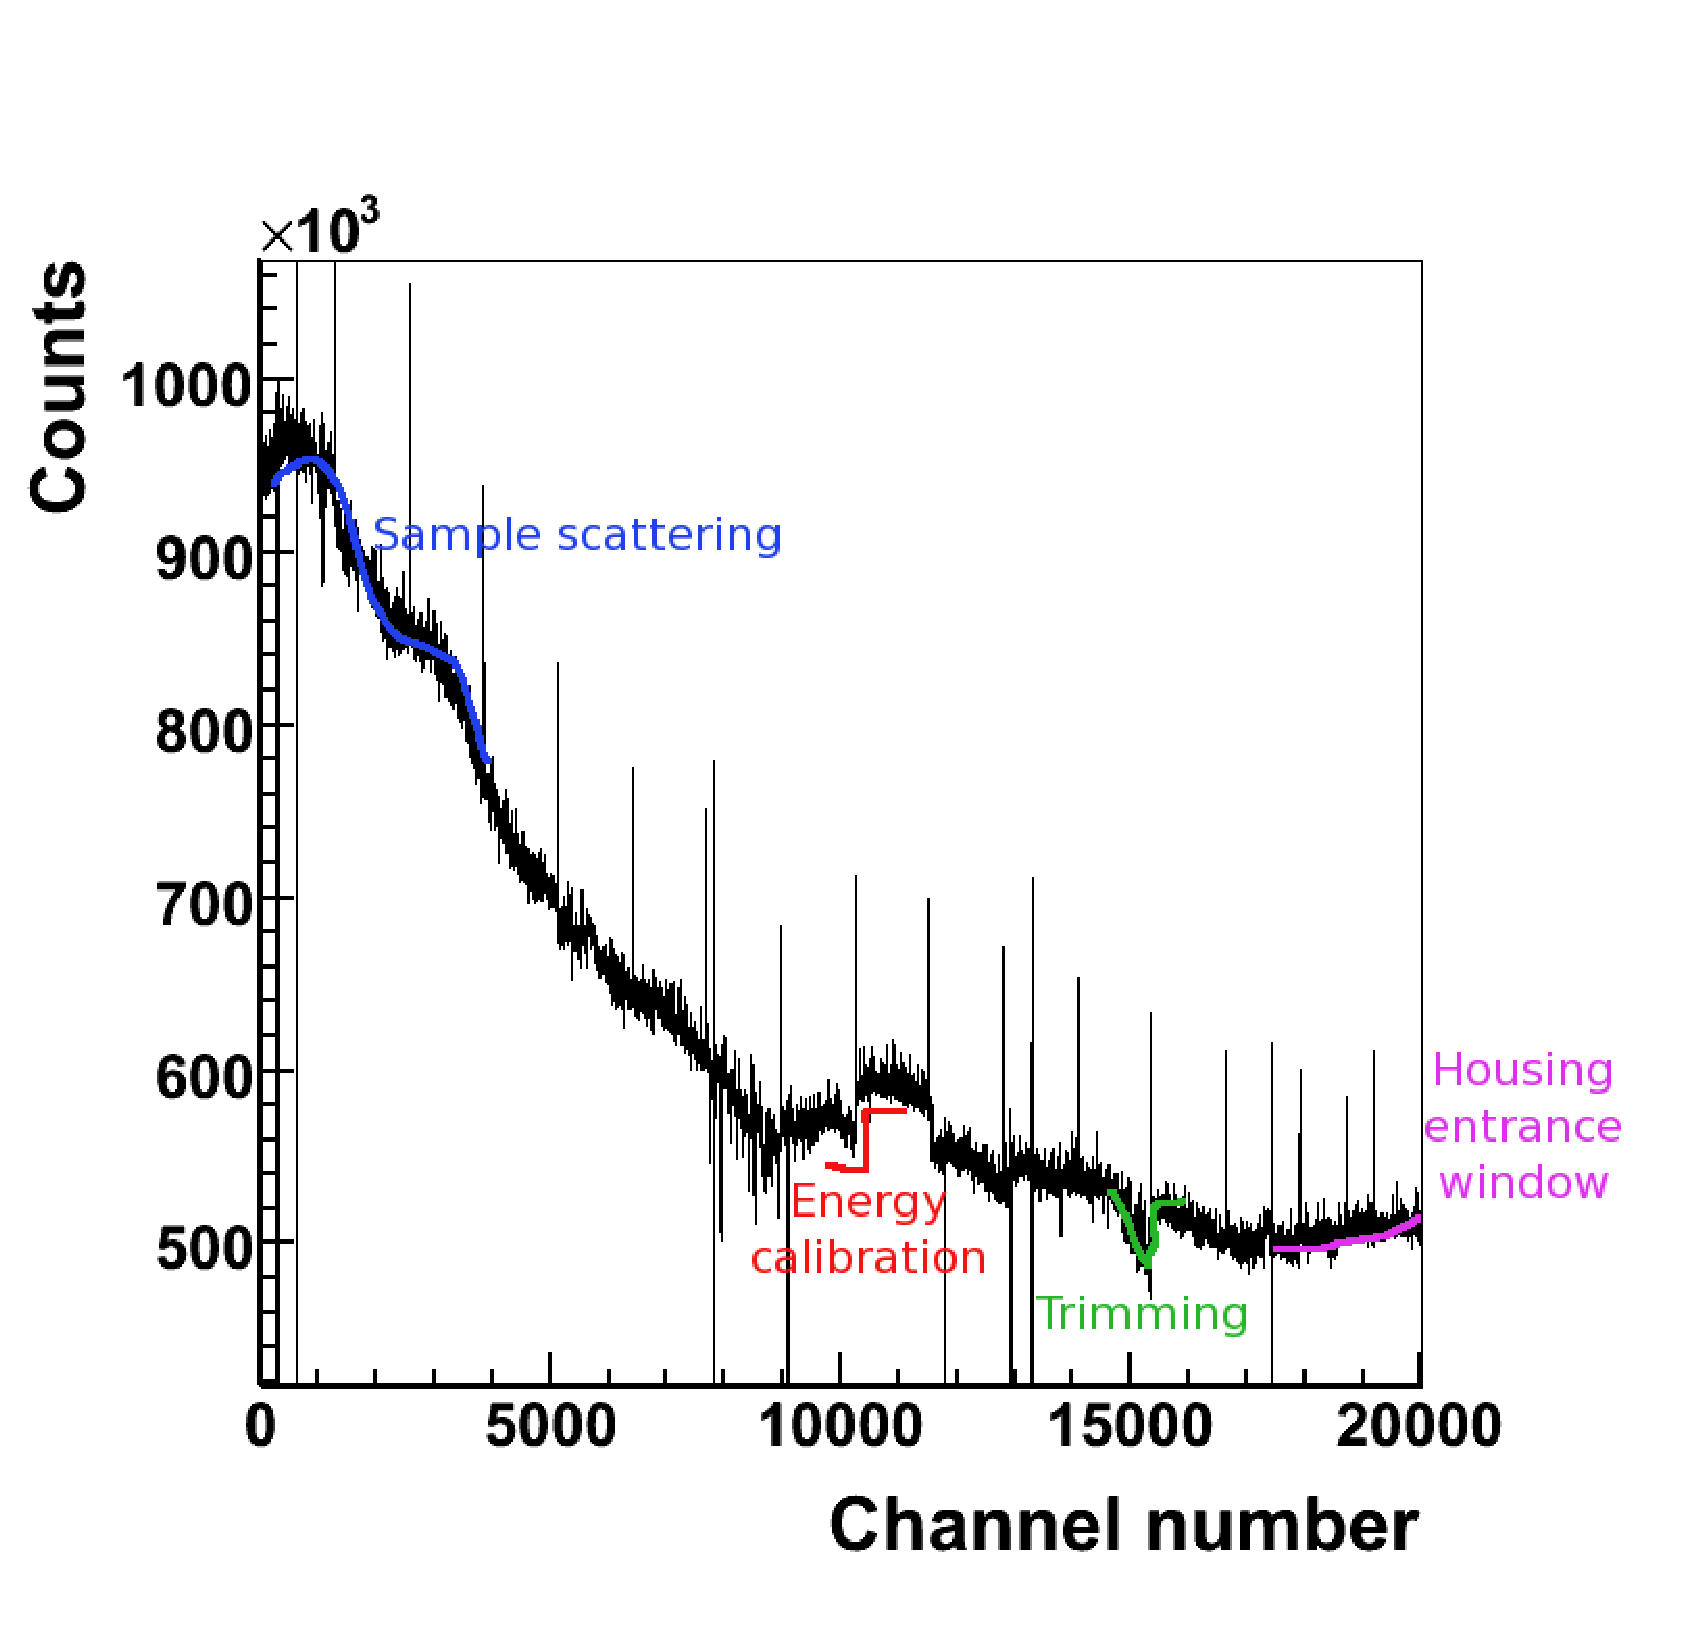
\includegraphics[width=\textwidth]{images/bad_ff_col}
\end{center}
\caption{Example of a very bad flat field data set with highlights of some of the reasons which can cause the non-flat behavior.}\label{fig:badff}
\end{figure}

\item The entrance window for the X-rays is deformed (we also have this problem at the SLS). In this case when you move the detector the "mountain" moves with it in angle (And remains still in channel number). However this should correct without problems with the flat field correction, even in case of fluorescent emission. Should appear at all energies.
\begin{comment}
\begin{figure}
\begin{center}
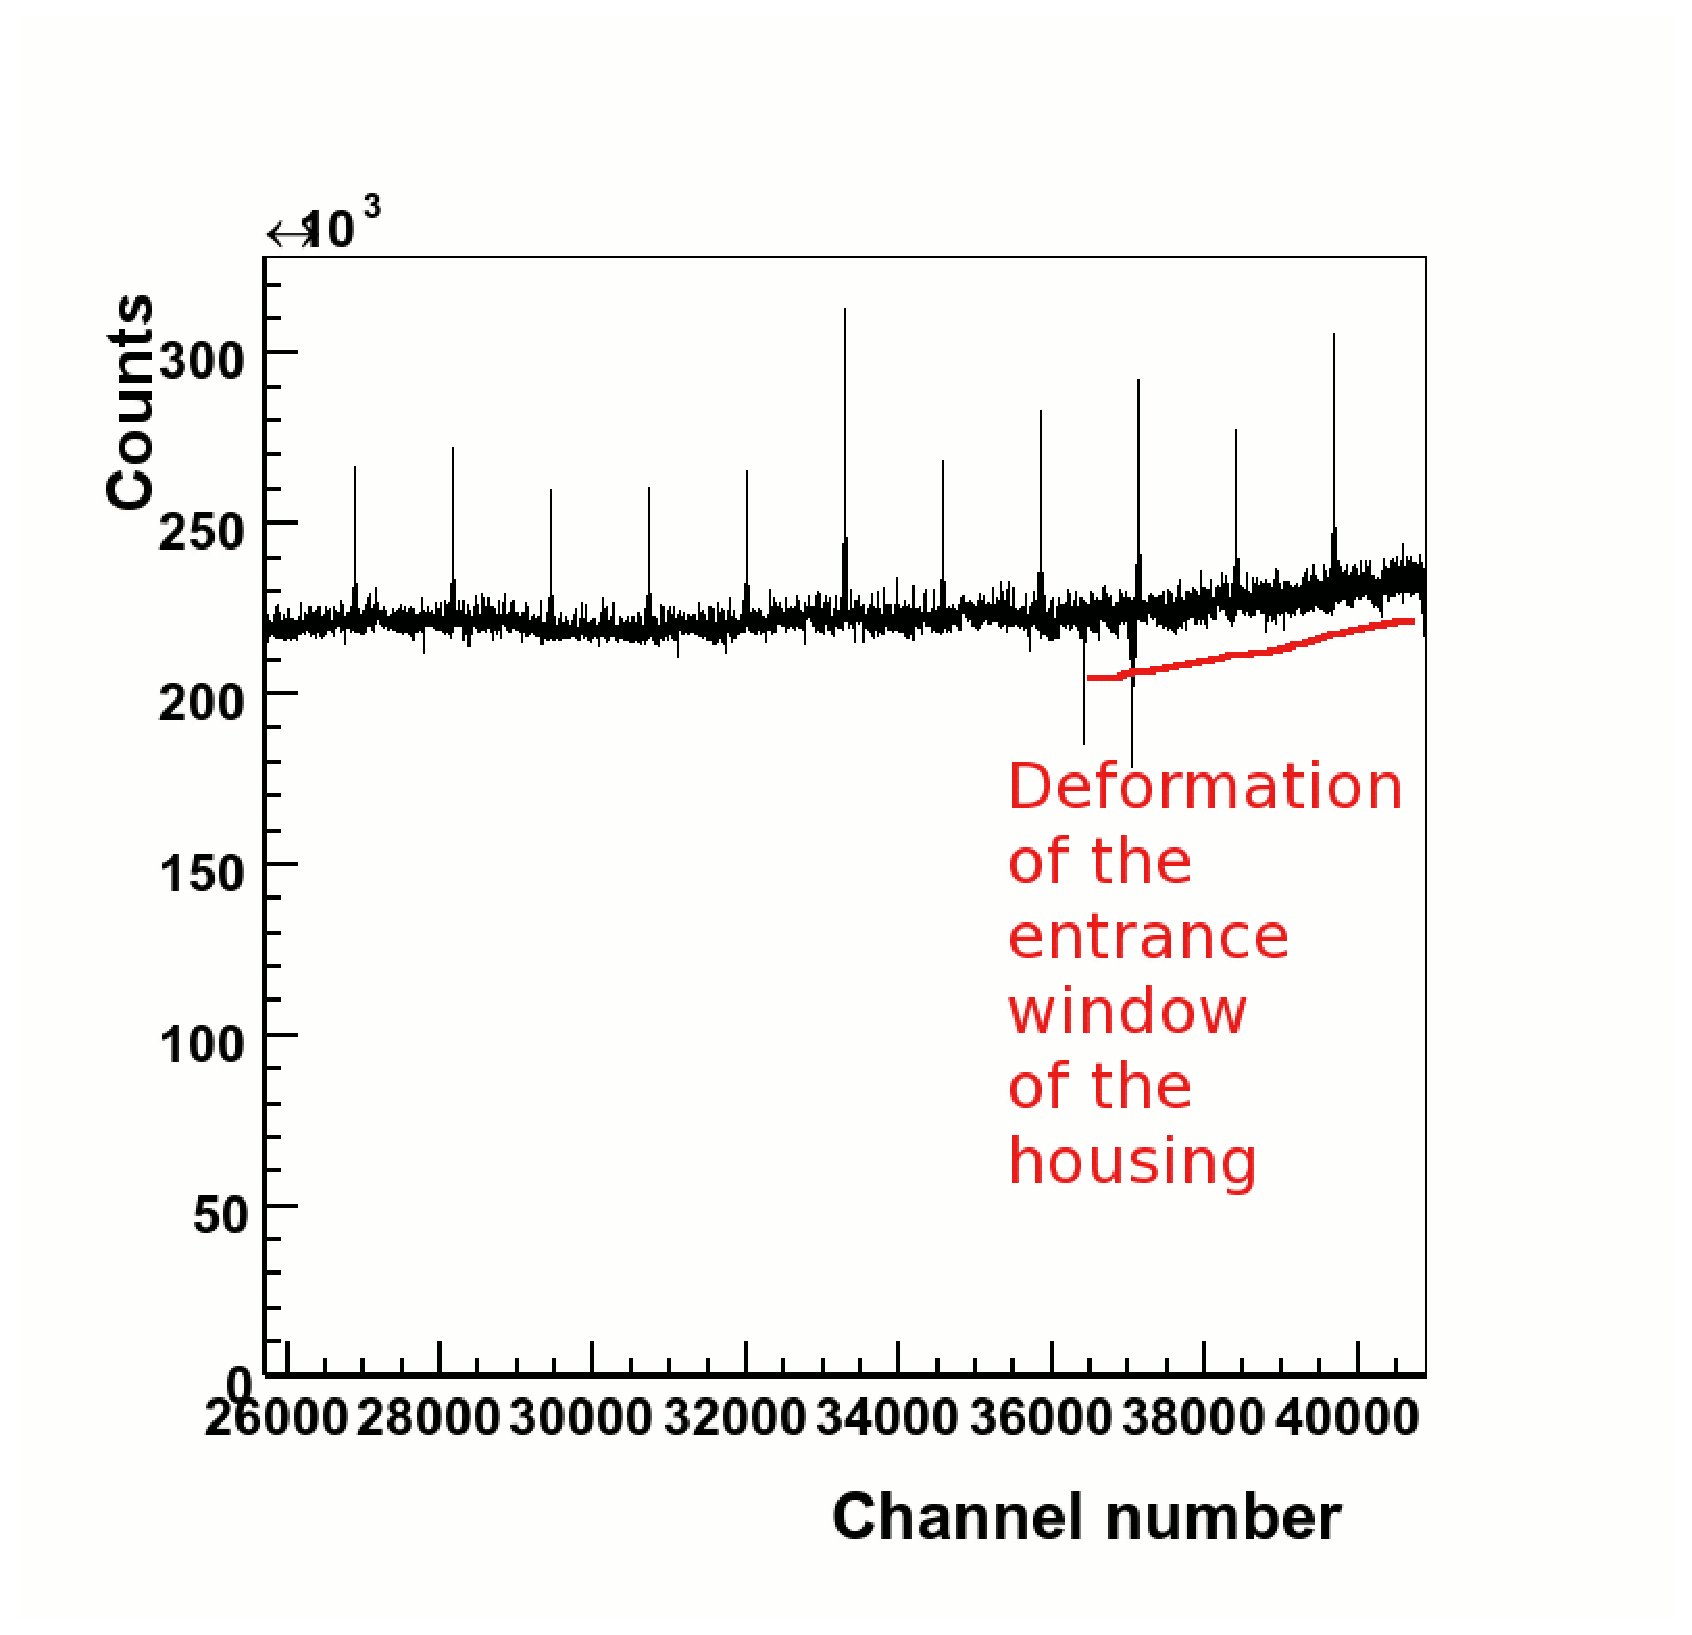
\includegraphics[width=\textwidth]{images/ff_window}
\end{center}
\caption{Variations in the flat field due to a non unifor entrance window of the detector housing.}\label{fig:ffwin}
\end{figure}
\end{comment}
\item Differences of efficiency between the modules i.e. mainly bad energy calibration. You normally see really steps at the transition between modules. Sometimes you have some groups of strips withing a module that are not properly trimmed and look as smallish peaks or valleys in the flat field. When you move the detector, these steps or peaks move in angle and remain still in channel number.
These differences can slightly change as a function of the energy (probably more evident at lower energies) but should normally always be there for the same settings.
These differences get much worse in presence of fluorescent emission, but normally correct properly with flat field correction.
\end{itemize}
\begin{comment}
\begin{figure}
\begin{center}
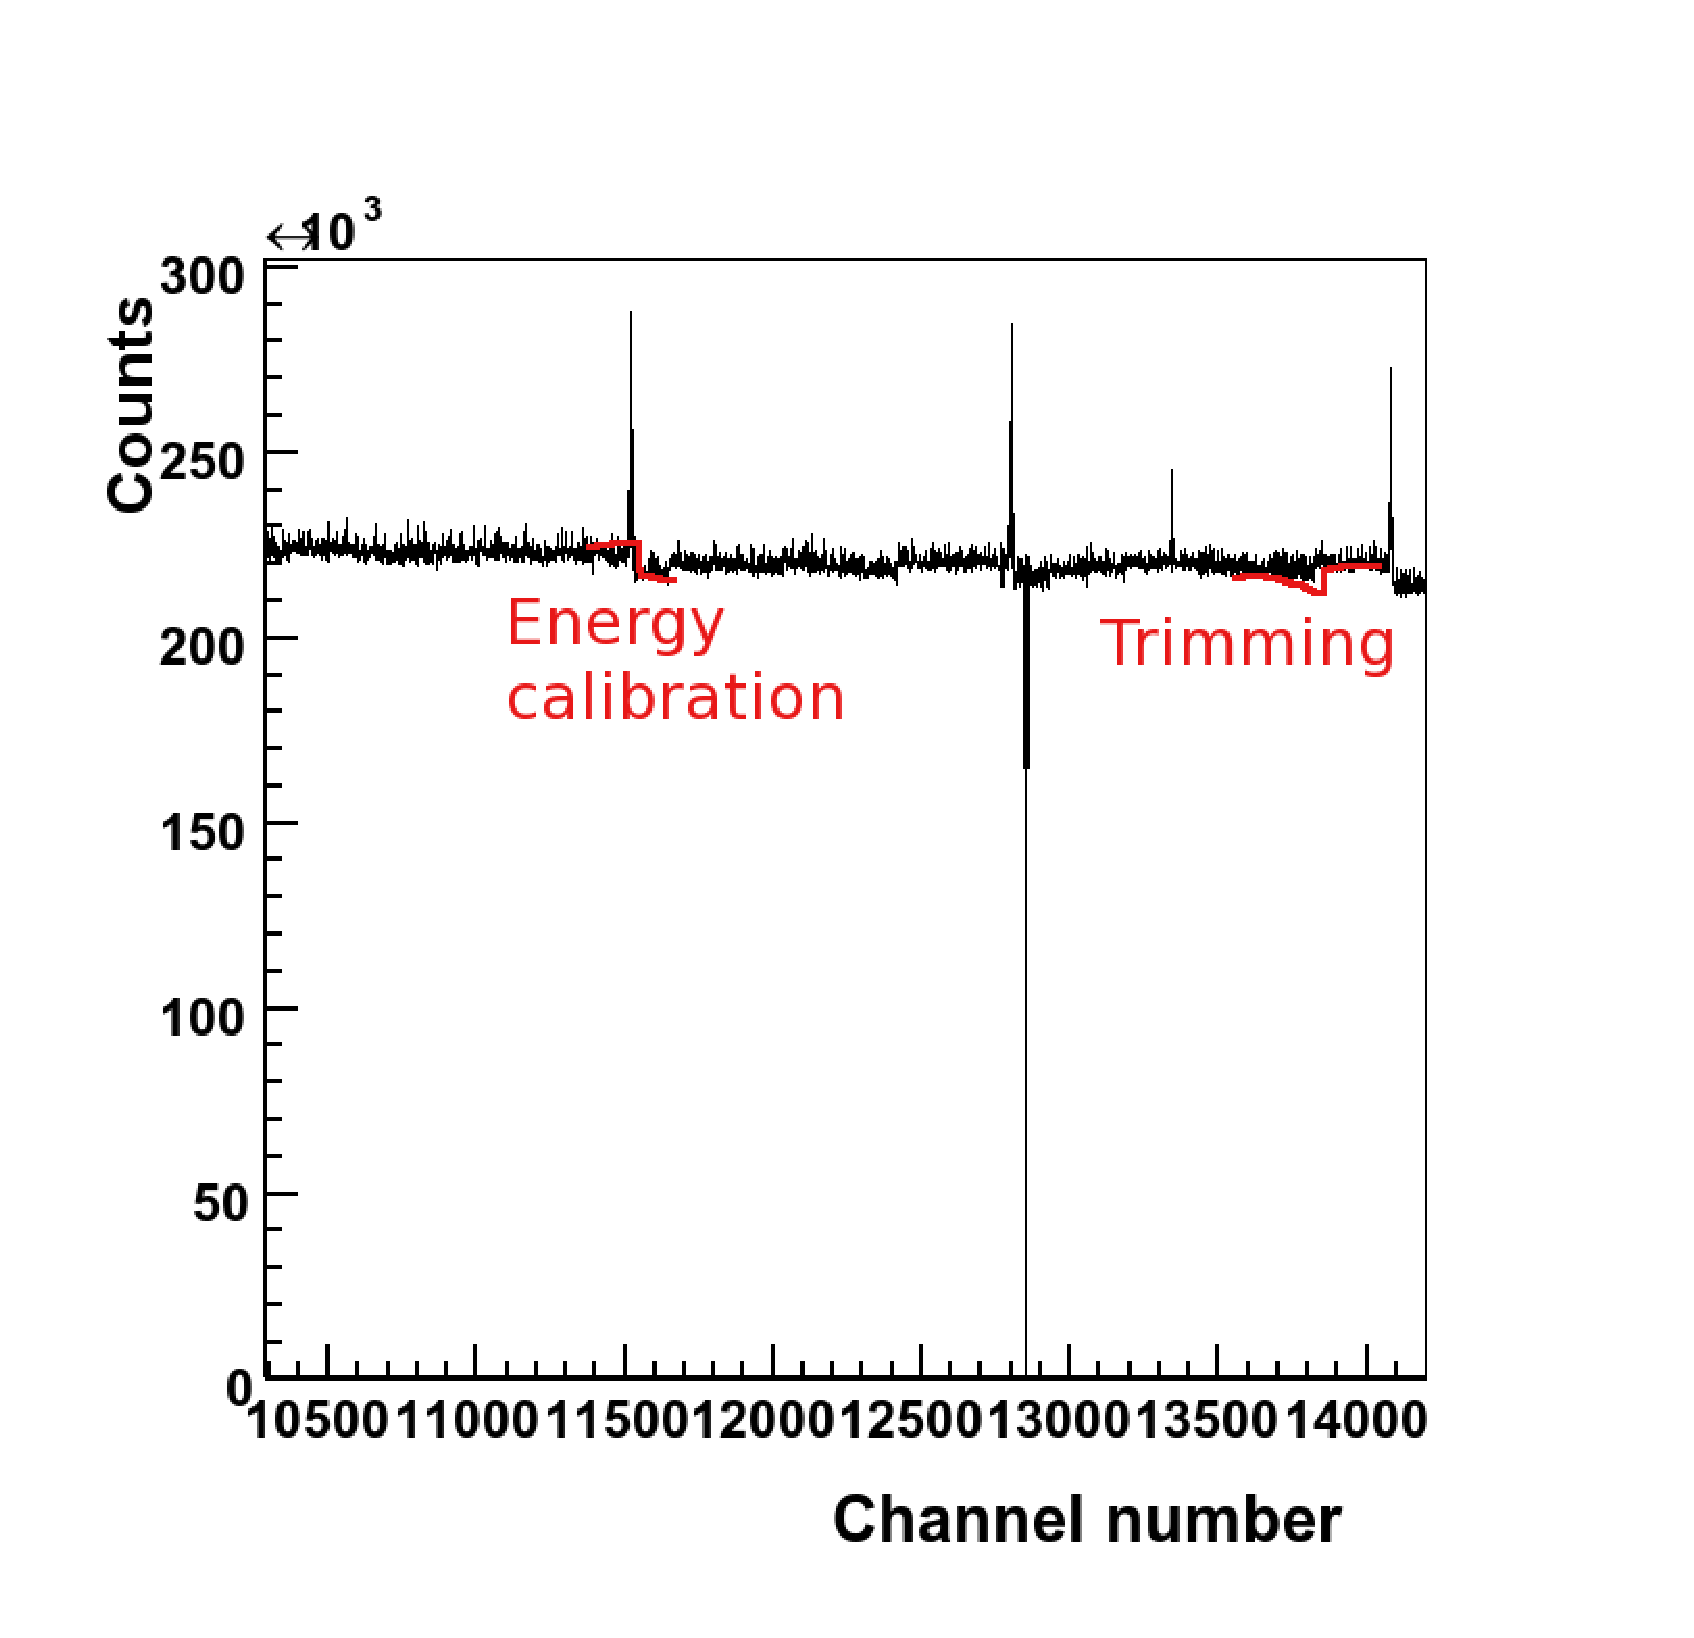
\includegraphics[width=\textwidth]{images/ff_calibration}
\end{center}
\caption{Variations in the flat field due to a non precise energy calibration or trimming of the detector modules.}\label{fig:ffcal}
\end{figure}
\end{comment}
\subsubsection{Dynamic acquisition of the flat field}

\begin{figure}
\begin{center}
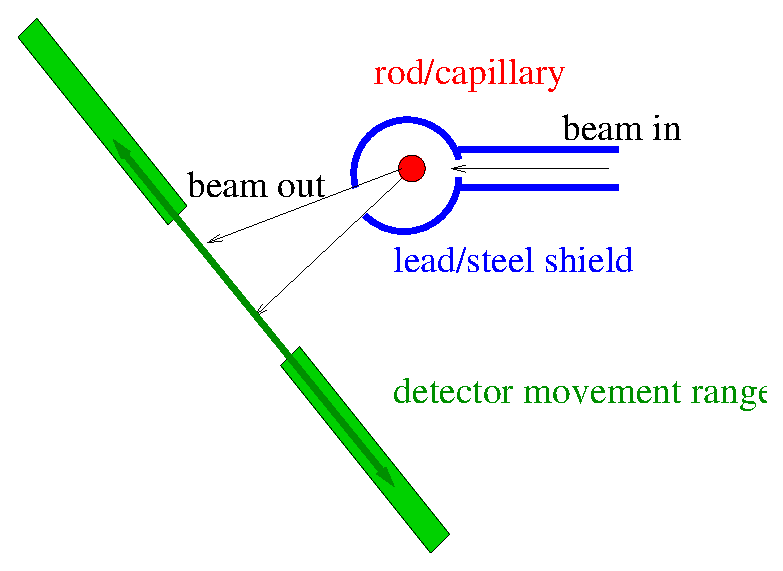
\includegraphics[width=\textwidth]{images/FFSetup}
\end{center}
\caption{Sketch of the experimental setup for a dynamic acquisition of the flat field.}\label{fig:ffsetup}
\end{figure}

\subsection{What happens when I trim the detector?}

General remarks about trimming.

\subsubsection{MYTHEN}

%\subsubsubsection{Trimming with noise} \label{sec:noisetrim}
\textbf{Trimming with noise} \label{sec:noisetrim}\\

The first step in the trimming procedure is to trim with noise (this is often sufficient). This has to be done for all the settings which are foreseen to be used (highgain, standard and fast).\\
The procedure for the noise trimming is as follows:
\begin{enumerate}
\item In the \textit{Initialization tab} click on the settings for which you want to trim (e.g. standard)
\item In the \textit{Initialization tab} click on the \textit{advanced} radio button to make the trimming accessible.
\item  In the \textit{Acquisition tab} set the acquisition time to 100~ms, the repetion to 1 and the delay between frames to 0.
\item For noise trimming usually the default parameters $Vthreshold=7$, $Counts=500$, $Resolution=4$ work.\\
However, to verify the threshold setting it is best to make a threshold scan. To do this go to the \textit{Data} tab, in the Data display section select the 2D color and type advanced option. In the \textit{Acquisition} tab select your data directory. Set the number of positions to 0. Select Scan, Type threshold. Typical values for the range are 500 to 900 with a step size of 10. Then click on the start button to perform the threshold scan. After the threhold scan has finished an image similar to the one in~\ref{fig:thresholdscanuntrimmed} should be shown. Depending on the system the number of modules may vary. If the plot is similar to the one in~\ref{fig:thresholdscantrimmed} the noise trim files did already exist and have been loaded when selecting the settings. In this case you don't need to trim with noise again.\\
Set the parameter Vthreshold in the \textit{Trimming} box (\textit{Initialization tab}) 10-30 DAC units below the onset of the noise for the module with the lowest threshold offset. Since the modules have differences in the offset and gain the onset of the noise varies. \\
You can usually leave the remaining parameters unchanged (Counts/pixel=500; Resolution=4).
\item Select the directory where the noise trim files should be written and the filename, to wich will be attached the extension given by the module serial number (.snxxx). If you want the trimfiles to be loaded authomatically when the global settings are selected, select the default directory specified in the config file (or in the ``trimbits/beamline'' directory for the older software versions). 
Click on \textit{Trim} to start the noise trimming process. After the trimming has finished look at the plot and the distribution of the trim bits. The distribution should be around 32$\pm$5 and should look gaussian. An example distribution is shown in figure~\ref{fig:trimdistribution} and an example plot in~\ref{fig:trimplot}. If the distribution is too much off center change the counts/pixel, if it is too narrow reduce the resolution (set it to 3), if it is too wide increase it (set it to 5). Make sure not too many channels have a trim value of 0 or 63.
\item Execute the treshold scan again to verify the trimming was done properly. A plot similar tho the one in figure~\ref{fig:thresholdscantrimmed} should appear.
\end{enumerate}

\begin{figure}
\begin{center}
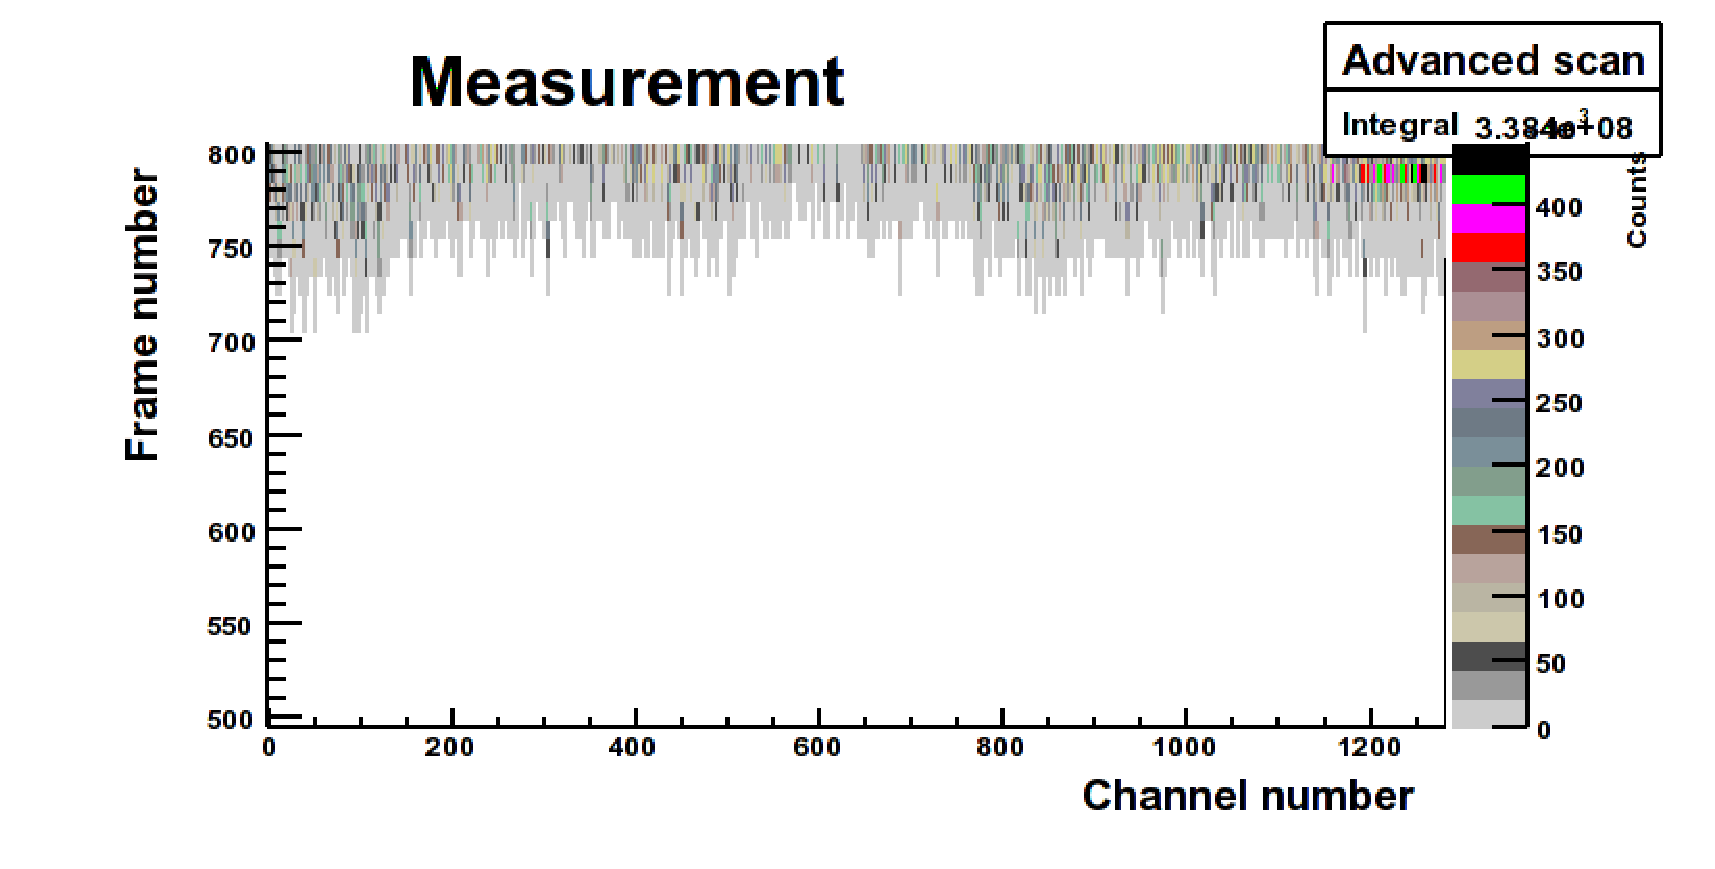
\includegraphics[width=\textwidth]{images/noise_thresholdscanuntrimmed}
\end{center}
\caption{The untrimmed threshold scan.}\label{fig:thresholdscanuntrimmed}
\end{figure}

\begin{figure}
\begin{center}
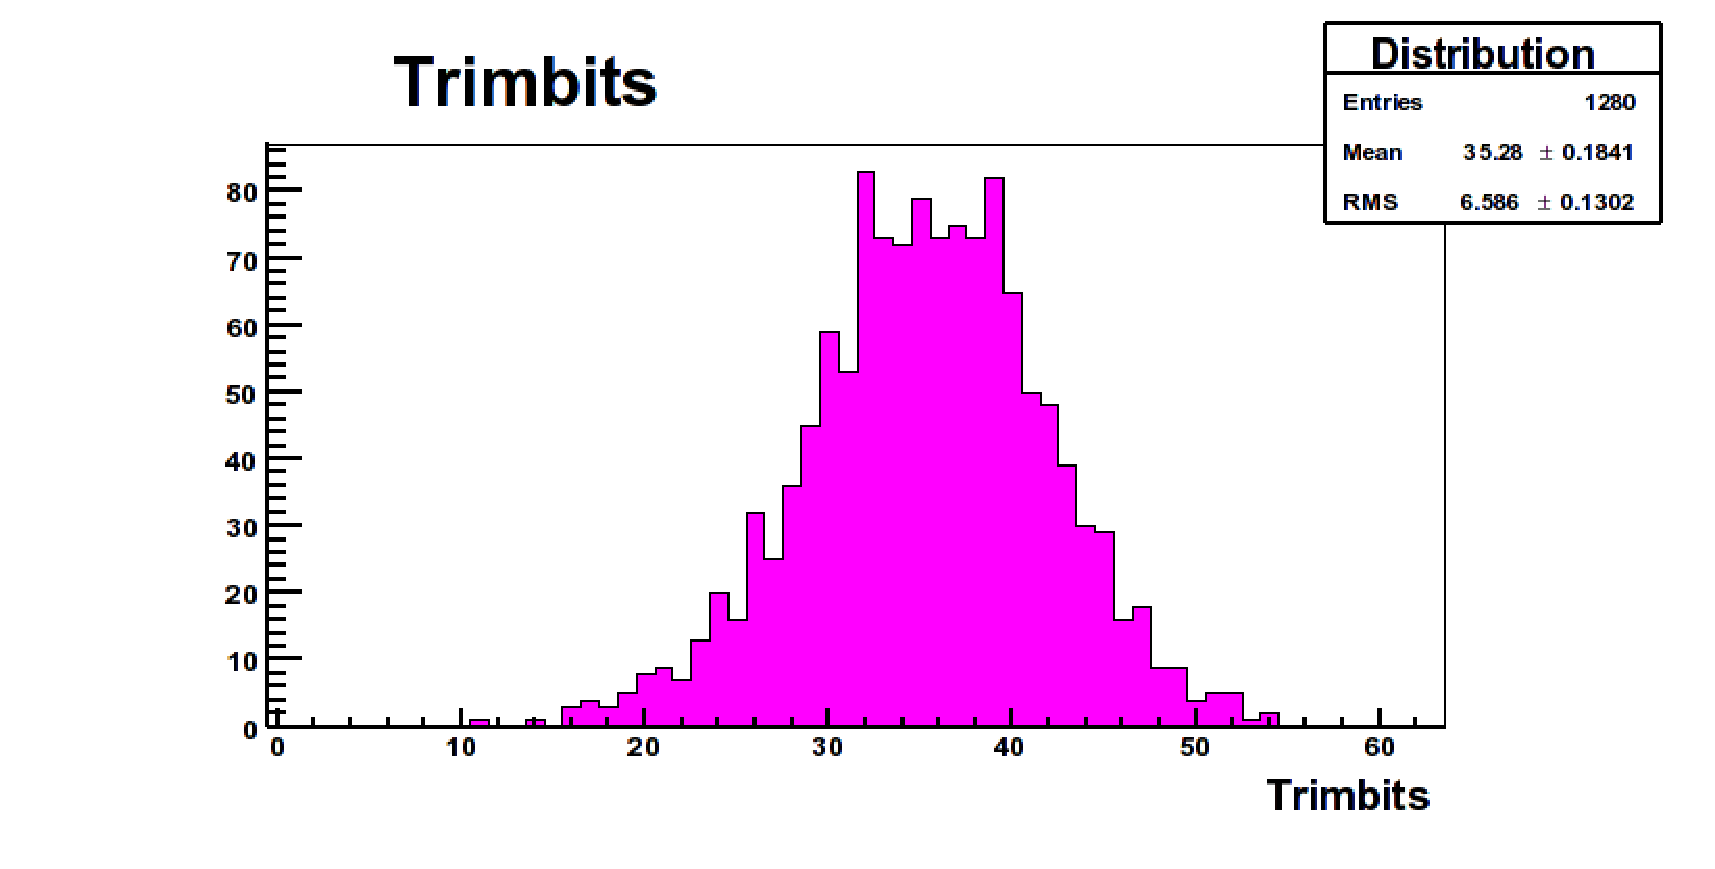
\includegraphics[width=\textwidth]{images/trimbitdistribution}
\end{center}
\caption{The distribution of the trimbits.}\label{fig:trimdistribution}
\end{figure}

\begin{figure}
\begin{center}
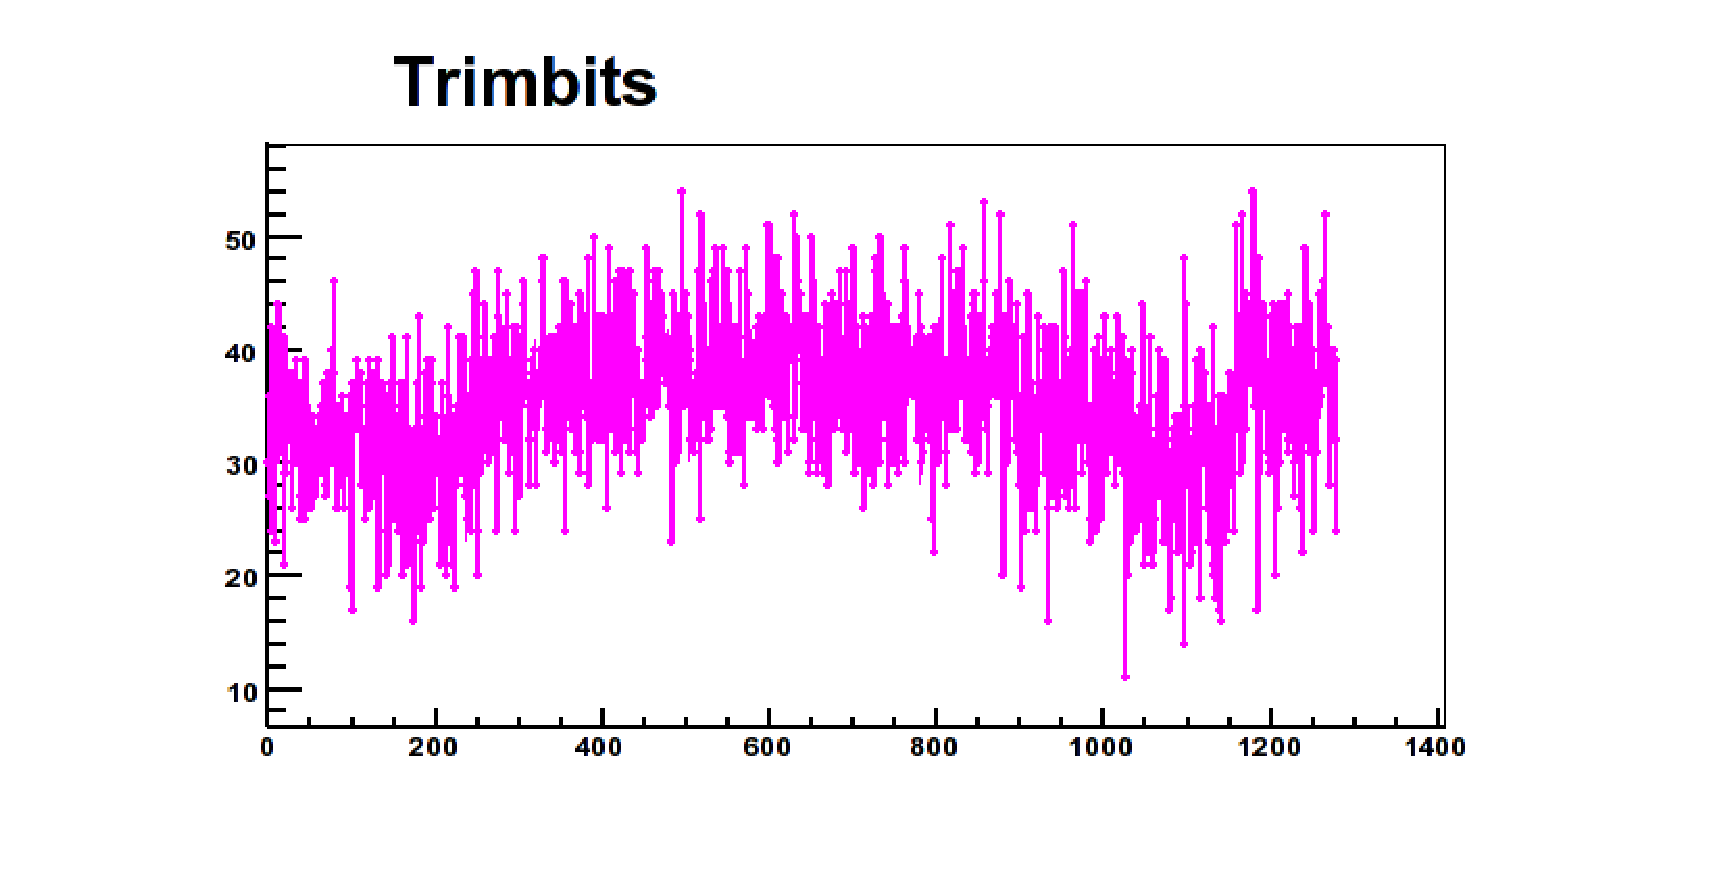
\includegraphics[width=\textwidth]{images/trimbitplot}
\end{center}
\caption{The trimbits for all the channels.}\label{fig:trimplot}
\end{figure}

\begin{figure}
\begin{center}
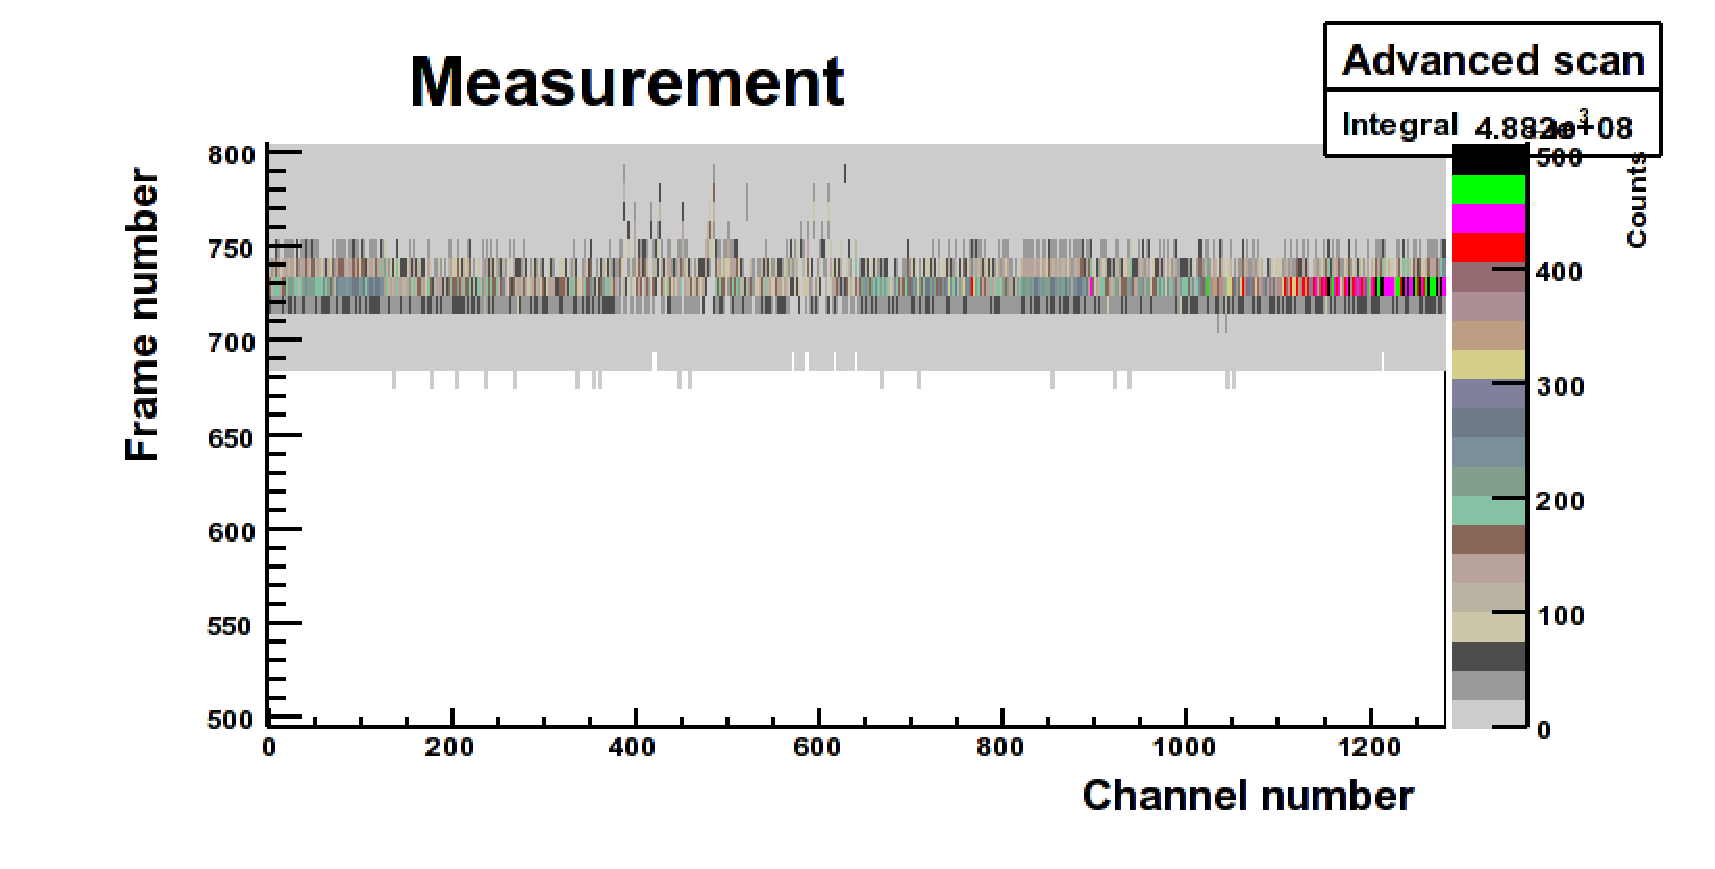
\includegraphics[width=\textwidth]{images/noise_thresholdscantrimmed}
\end{center}
\caption{The trimmed threshold scan.}\label{fig:thresholdscantrimmed}
\end{figure}
\textbf{
%\subsubsubsection{
Improve the trimming using X-rays}\label{sec:improvetrimming}\\

The improvement of the trimming acquired with noise is not essential: at 12~keV an untrimmed module has a threshold dispersion which is about 1.4~keV and is already reduced to 200~eV at 12~keV by the noise trimming. At lower energies the noise trimming will be more effective, while the threshold dispesion will be still larger at higher energies. The trimming improvement reduces the threshold dispersion to 140~eV at 12~keV and is expected to be almost constant at all energies. For this reason it is suggested to perform the trimming improvement only when a small threshold dispersion is really important (e.g. to avoid flat field corrections or in presence of fluorescent lines close to the threshold value) and it will probably be not worthy at lower energies (i.e. threshold lower than 6~keV and X-ray energy lower than 12~keV). 
The procedure for the trimming improvement is as follows:
\begin{enumerate}
\item Select the settings of the detector and load the noise trimming file
\item Set the threshold at half of the X-ray energy (better if the detector has already been calibrated in energy like explained in~\ref{sec:encal})
\item Illuminate the detector with a flat field. This is very important to obtain a good trimming. 
\item Select the \textit{acquisition time} in the \textit{acquisition tab} so that there are at least 1000 counts/strip per frame (the more counts, the better trimming). Set the repetions to 1 and the delay between frames to 0.
\item Go to expert mode by clicking on \textit{advanced} in the \textit{initialization tab}, \textit{settings} box
\item In the trimming box  select the directory where the noise trim files should be written and the filename, to wich will be attached the extension given by the module serial number (.snxxx).
\item Select the \textit{improve} method
\textit Start the trimming
\end{enumerate}
If the trimming is correctly performed and the illumination is flat enough, the same trimming can be used every time you will measure at this same energy.
The authomatic loading of energy-specific trim files is not yet implemented.

\subsection{In what consists the energy calibration of the detector?}\label{sec:encal}

General remarks about DAC to energy conversion

\subsubsection{MYTHEN}

Since the conversion between the threshold DAC units and energy depends on the gain and offset of the channels the energy calibration has to be done for all settings (high gain, standard and fast). For each setting follow this procedure:
\begin{itemize}
\item Select the setting in the \textit{Initialization} tab.
\item Enter in expert mode by clicking the \textit{Advanced} radiobutton in the \textit{Global settings} box in the \textit{Initialization} tab.
\item If the trimfiles are in the correct location and with the correct name, they should be loaded by default every time you select the corresponding settings in the \textit{global settings} box in the \textit{initialization} tab~\footnote{The default name of the calibrated trimfiles is \textsf{trimbits/beamline/}\textit{settings}\textsf{/noise.snxxx} where  \textit{settings} is the chosen settings. You  can change it in \textsf{src/qDetector.h} and then recompile the acquisition program as described in~\ref{sec:installation}.}.
If the trim files do not yet exist generate them as explained in section~\ref{sec:noisetrim}.
\item Execute a threshold scan of the detector with at least three different energies. The more monochromatic are the X-rays, the better the calibration will be (i.e. scattered X-rays are better than the fluorescent emission). \\
The scan should range from where all modules count 0 (estimate 850-20$\cdot$energy(keV) DAcu) and where all modules start having a lot of noise (usually 800 DACu) with a step of 1 or 2 DACu. The acquisition time should be chosen so that there are at least 1000 counts per strip on the plateau.
\item Open the file \textsf{root/CalAllModules.C} for editing. Change the value of the following global variables according to your needs:
\begin{itemize}
\item \textit{nmod} is the number of modules of your system.
\item \textit{nscan} is the number of different threshold scans you acquired.
\item \textit{en} is the array with the energies at which you acquired the scans, in keV.
\item \textit{een} is the array with the errors on the energies at which you acquired the scans, in keV. It is usually small, but can be some hundreds eV in case of dirty fluorescent samples.
\item \textit{fn} is the array containing the location and root file name of your data.
\item \textit{run} is the array containing the run index of your data.
\item \textit{startscan} is the array containing the threshold value at which you started the scans.
\item \textit{stopscan} is the array containing the threshold value at which you finished the scans.
\item \textit{stepscan} is the array containing the threshold step of the scans.
\item \textit{ave} is the array containing the average number of counts per strip on the plateau (it must not be too precise).
\item \textit{sn} is the array containing the list of the serial number of the modules to be calibrated. It is important that the list is in the right order, so that the optput calibration files have the extension .snxxx corresponding to the right module.
\item \textit{of} is the location and root file name of the calibration file. The directory should already exist and the extension .snxxx will be attached to the output file.  
\end{itemize}
\item Launch \textsf{root}, which you should have already installed on your linux PC
\item Execute the following commands in order to load the macros needed for the calibration:
\begin{verbatim}
root$ .L root/NewMythenMacros.C++
root$ .L root/CalAllModules.C++
\end{verbatim}
You should get a lot of warnings, but no errors.
\item Execute the following command in order to run the calibration:
\begin{verbatim}
root$ EnCalModules()
root$
\end{verbatim}
Reading and analyzing the data takes some time, but, after a while, a canvas should open where the plots of the median of the counts of every module as a function of the threshold should be shown for each energy, fitted with a modified \textit{erf} function in order to find the inflextion point. The last plot of the canvas should represent the inflexion points as a function of the energies, and by fitting it with a straight line it is possible to calculate the offset and gain for each module i.e. calibrate it as a function of the energy. Please check that this automated fitting procedure succeeds. In case you see many fitting errors you should try to check wether the variable you edited in  \textsf{root/CalAllModules.C} are all correct or try to edit the fitting procedures in the two root macro files (sorry!).
\item Copy the calibration file you obtained to \textsf{calibration}/\textit{settings}\textsf{.snxxx}~\footnote{The default name of the calibration file \textsf{calibration/}\textit{settings}\textsf{.snxxx} where  \textit{settings} is the chosen settings. You  can change it in \textsf{src/qDetector.h} and then recompile the acquisition program.} By doing this the correct threshold for each module will be calculated every time you change the \textit{threhsold energy} in the \textit{global settings} box in the \textit{initialization} tab, you have loaded some default settings and you are not in expert mode.  
\end{itemize}

\subsection{Why should I change the dynamic range of the counters?}

\subsection{When should I enable rate correction}
\subsubsection{How can I choose the dead time?}


\section{Analog detectors}

Various issues concerning calibration, dynamic gain switching, data handling data processing etc.
\subsection{(Dynamic) Gain Switching}
\subsection{Pedestals}
\subsection{Energy calibration}
\subsection{Data processing}




\section{Angular conversion}


\subsection{How is the channel number coverted into angle?}\label{sec:angcal}


Mythen II modules are composed by 1280 pixels, each having width p = 0:05 mm, and numbered with j = 0; : : : ; 1279.
Angles are counted counterclockwise from the beam direction. For the m-th module, the angle jm of its j-th pixel
center can be determined using the three geometric parameters Rm [mm], m [deg], Dm [mm], as in Fig. 1. The
detector group uses instead the 3 parameters center cm [ ], oset om [deg], conversion km [ ]. The law with the 3
geometric parameter is
jm = m �

180


arctan

Dm � pj
Rm

(1)
1
The corresponding law using DG's parameters is
jm = om +

180


cmkm +

180


arctan [(j � cm)km] (2)
One can convert the two forms by equating separately the term out of the arctan and the argument of arctan for two
dierent values of j. It results
cm =
Dm
p
; (3)
km =
p
Rm
; (4)
om = m �
180

Dm
Rm
: (5)
Conversely,
m = om +
180

cmkm; (6)
Rm =
p
km
; (7)
Dm = cmp: (8)
2

This section is specifically (but not only) for larger systems for powder diffraction. It is assumed that the scripts for moving the detector axis have been adopted to the beamline (see chapter~\ref{cha:integration}). For the angular calibration a Si sample is mounted and the detector is moved in steps of 0.1 deg over the 111 peak. Afterwards the recorded data has to be analyzed to produce the angular calibration file. 
The procedure for the data taking is as follows:
\begin{enumerate}
\item Setup the detector trimmed with the correct settings (not important which) an the threshold at half of the X-ray energy.
\item Mount the silicon capillary and select the acquisition time to verify that the peak has a height of more than 5000 counts. Make sure the detector is operated in the linear region of the count rate, otherwise use more filters and a longer acquisition time. The energy is not very important, but it should not be very low (>10~keV). 
\item Move the detector to the angular position such that the Si111 peak is just before the first module. 
\item Select both header before and header after (the detector position needs to be written in the header files!) and click on \textit{scan}, \textit{before each frame} selecting a scrip that moves the motor. In the scan variable range set the start position such that Si111 peak is just before the first module, the stop position when the Si111 peak is already out of the last module (e.g. start position - (detector range +5)) and a step of 0.1 deg.
\item Start the acquisition. It is very likely that if your detector is large it will take several minutes or even hours.
\end{enumerate}

Edit the script \textit{angcal.awk} and set the STARTPOSITION variable to the current position. In the \textit{Acquisition} tab set the number of positions to 0, scan, type none, script before frame and with the Browse button select angcal.awk. Set scan from to 0. To should be a few degrees more than 10x the angular coverage of the detector (e.g. 950 for a 90deg detector). This is because the detector is stepped in steps of 0.1 deg. The step size should be 1. For this example the number of steps should be 950. Press start to begin the data taking. After data taking has finished open a terminal, go to the directory where the data is and start root.

For the data analysis (will be upgraded):
\begin{enumerate}
\item Start root
\item Edit the file \$MYTHENDIR/root/convertNewMythenIInew.C to match your setup (epics variable, direction etc.)
\item Load the macro file convertNewMythenIInew.C:

\texttt{root\$ .L  \$MYTHENDIR/root/convertNewMythenIInew.C+}

\item Run the analysis function: 

\texttt{root\$ fitangle(fname,extension, start, stop, startangle, stopangle);}
 
where fname is the file name (with complete path), extension should be ``.raw'', start is the start position, stop is the stop position, start angle should be the position of the silicon peak -0.5 deg and stop angle the position of the silicon peak +0.5 deg.

\item The procedure will produce a file ang.off containing the angular calibration coefficients for your detector. Copy it to your default location and set it in the config file of the GUI (see section~\ref{sec:configtxt}).


\end{enumerate}


\subsection{How are different positions merged together?}\label{sec:merging}

\subsubsection{Why can't I properly merge different positions?}

From my experience, when data don't merge properly after flat-file corrections there are mainly two reasons:
\begin{itemize}
\item FLUORESCENCE. We ahve already discussed about it and normally it shouws up as differences between individual channels or groups of channels i.e. the patterns don't match in several places.
This does not seem the case, in my opinion (but do you know exactly what's inside Aspirin?)

\item Background scattering from the air. When you move the detector the walls of the housing make a different shadow on the modules and at small angles if you have no beamstopper it could even be backscattering from the housing hit by the beam in the different positions. The only way of improving it is to properly place the beamstopper and to avoid air scattering before the sample e.g. by using a "nose" from the end of your flight tube to very close to the sample.
Of course the problem is stronger at lower energies (more air scattering) and normally with the detector positioned at low angles (scattering from the housing, shadowing of the "forward" scattered beam).
When you see this problem you could try to take data e.g. at 20-25 degrees instead of 5-10 degrees and see if it's still there.
It could also be that the geometry of your housing with the flat window and shorter path inside the housing amplifies the problem, so that you should take special care of it with respect to the SLS where we have just a feww cm before entering the housing and then half a meter inside it.

\item Your sample changes over time e.g. in case of radiation damage and long exposure times (usually several seconds).

\end{itemize}


\end{document}
